\chapter{Extension of the Rule-Based Lloyd Algorithm to 3D\label{chap:rbl}}
\section{Introduction}
    \subsection{Motivation}
        Motivation in using \ac{RBL} algorithm offers communication-less approach for guiding multiple agents from point A to point B.
        It requires an estimate of its position—whether through \ac{GPS}, \ac{RTK} or methods like \ac{SLAM}—along with onboard sensors that provide information about the surrounding environment, enabling it to avoid obstacles and move toward the goal.
        So far, the algorithm has mainly been tested in \ac{2D} scenarios with a fixed altitude, and the results have looked promising. 
        This were the main motivation factors to try and extend it to full \ac{3D} navigation, where altitude and sensor orientation also play a role.

    \subsection{Problem Statement}
        Many real-world robotic applications, particularly involving \ac{UAV}, require navigation within \ac{3D} environments containing obstacles. 
        While algorithms like the \ac{RBL} \cite{rbl_paper} have proven effective in \ac{2D} goal convergence, they are inherently limited when applied directly to \ac{3D} space. 
        The core problem arises because the existing \ac{RBL} algorithm is fundamentally designed for \ac{2D} planar navigation, making it unsuitable for applications like UAV operations that require navigating in \ac{3D} space.
        Specifically, there is a need to extend existing \ac{2D} algorithms to \ac{3D} while smartly incorporating vertical exploration to ensure safe, efficient, and effective navigation through crowded 3D environments without significantly compromising performance or requiring excessive computational resources. 
        This work addresses the challenge of adapting the \ac{RBL} algorithm for \ac{3D} space by developing and evaluating specific rules to control vertical movement, aiming to achieve robust 3D navigation capabilities.
        
    \subsection{Objectives}
        \begin{itemize}
            \item   Enhance the convergence speed of agents towards their goals by promoting exploration, with  focus on the vertical exploration.
            \item   Demonstrate the algorithm's enhanced applicability, achieved by extending goal placement to the z-axis.
        \end{itemize}

    \subsection{Chapter Overview}
        The principles of the \ac{RBL} algorithm, presented in \cite{rbl_paper}, form the basis of the work in this chapter. 
        These principles are clarified and modified to address the challenges of \ac{3D} extension.  
        The chapter details the fundamental principles of RBL in \ac{2D} and \ac{3D} spaces, describes the specific rules applied to enhance convergence, and concludes with a series of simulation scenarios designed to demonstrate the performance of the proposed solution.
        Finally, the chapter concludes in the presentation and evaluation of simulation experiments designed to assess the efficiency of the proposed \ac{3D} extension and the impact of the introduced vertical exploration rules.

\section{Basic principles of Rule-Based Lloyd Algorithm}

    \subsection{Overview}        
        The algorithm is a communication-less approach designed to navigate agents from point A to point B. 
        The algorithm's ability to determine each agent's position relative to its goal depends on the availability of positioning data. 
        This can be either global positioning data, such as from GPS, or relative positioning data obtained through techniques like SLAM in GNSS-denied environments, combined with sensor inputs that provide information about the agent's surrounding environment.
        These sensors can include LiDAR, depth cameras, or standard cameras with estimation techniques, allowing the agent to detect and avoid obstacles or other agents. 
        The algorithm enables autonomous navigation without requiring direct communication between agents, making it suitable for scalable and decentralized applications.

    \subsection{Applications and Limitations in 2D}
        Modern robotics relies on the capability to navigate from point A to point B.
        Navigation plays a crucial role in various robotic applications, such as \ac{UGV}s, which are commonly used in manufacturing and logistics. 
        \ac{UGV}s typically follow predefined \ac{2D} trajectories guided by visual \cite{vision_navigation}, magnetic \cite{magnetic_navigation}, or LiDAR-based navigation \cite{lidar_navigation}. 
        Additionally, \ac{2D} navigation is widely used in robotic vacuum cleaners, enabling them to systematically cover an area while avoiding obstacles.

        An obvious limitation for algorithms in \ac{2D} is scalability. 
        As the number of agents in a system increases, the complexity of managing their movements and coordination also grows significantly.
        Obstacle avoidance in \ac{2D} can also be less efficient compared to \ac{3D} environments, as agents have fewer options for evading obstacles. 
        In \ac{3D}, agents can change their altitude in addition to their horizontal trajectory, giving them more freedom to maneuver around obstacles.

    \subsection{Key Principles in 2D}
        It should be noted that most of the infromation presented here is adapted from the work detailed in \cite{rbl_paper}.
        RBL ensures convergence to the goal and provides sufficient conditions for achieving it. 
        The problem involves individual control of $N$ agents from their initial position $\mathbf{p}_i(0)$ toward a goal region, represented as circle.
        This goal region is denoted as $G(\mathbf{g}_i, r_g)$, where $\mathbf{g}_i$ is center and $r_g$ is radius of goal region. 
        The agent is progressing towards its designated destination, $\mathbf{d}_i$.
        Each agent knows its current position $\mathbf{p}_i$, encumbrance $\delta_i$, which determines safe space around agent.
        Additionally, each agent also knows the positions and encumbrances of its neighboring agents $\mathbf{\mathcal{N}_i}$, agent $j \in \mathbf{\mathcal{N}_i}$ if $||\mathbf{p}_i - \mathbf{p}_j|| \leq \frac{r_{s,i}}{\eta}$, where $r_{s,i}$ is sensing radius of the i-th agent and $\eta$ is a scaling parameter of cells.
        For simplicity $r_{s,i}$ is considered to be same for all agents, therefore $r_{s,i} = r_s$. 

        The core objective of the algorithm is to maximize the coverage cost function, which accounts for the distribution of agents and obstacles over the environment. 
        This function is expressed as:
        \begin{equation}
            J_{cov}(\mathbf{p}) = \sum_{i=1}^{N} \int_{\mathcal{V}_i} \lVert\mathbf{q}-\mathbf{p}_i\rVert^2 \varphi_i (\mathbf{q})d\mathbf{q},
            \label{coverage_cost_function}
        \end{equation}
        where $\mathbf{p}_i$ is the position of agent $i$, $\mathcal{V}_i$ is the Voronoi cell of the i-th robot, $\lVert\mathbf{q}-\mathbf{p_i}\rVert^2$ is squared Euclidian distance between point in the mission space $\mathbf{q} \in \mathcal{Q}$ and agent's position $p_i$, 
        and $\varphi_i (\mathbf{q})$ is the weighting function.

        Voronoi cell is defined as: 
        \begin{equation}
            \mathcal{V}_i = \{q \in \mathcal{Q} \lvert \lVert \mathbf{q} - \mathbf{p}_i \rVert \leq \lVert q - \mathbf{p}_j \rVert, \forall j \neq i\}
        \end{equation}
        For visual representation see \reffig{fig:voronoi_2d}. 

        However, this standard definition of Voronoi cells does not take into account the physical space occupied by the agents, their encumbrances. 
        To address this, a Modified Voronoi cell is introduced, which takes into account the encumbrances of agents.
        This modified version adjusts the boundaries of each Voronoi cell to account for the encumbrances of neighboring agents.
        Also to enhance the algorithm performance, the Voronoi cell are scaled using a scaling parameter $\eta \in [0, 1]$.
        The modified Voronoi cell definition is as follows:
        \begin{equation}
            \label{eq:voronoi_cell_account_encum}
            \tilde{V}_i = 
            \begin{cases}
            \{ \mathbf{q} \in Q \mid \| \mathbf{q} - \mathbf{p}_i \| \leq \eta \| \mathbf{q} - \mathbf{p}_j \| \}, & \text{if } \Delta_{ij} \leq \frac{\| \mathbf{p}_i - \mathbf{p}_j \|}{2} \\
            \{ \mathbf{q} \in Q \mid \| \mathbf{q} - \mathbf{p}_i \| \leq \eta \| \mathbf{q} - \tilde{\mathbf{p}}_j \| \}, & \text{otherwise},
            \end{cases}
        \end{equation}
        $\forall j \in \mathcal{N}_i$, where $\Delta_{ij} = \delta_i + \delta_j$ and $\tilde{\mathbf{p}}_j = \mathbf{p}_j + 2(\Delta_{ij} - \frac{\| \mathbf{p}_i - \mathbf{p}_j \|}{2})\frac{ \mathbf{p}_i - \mathbf{p}_j }{\| \mathbf{p}_i - \mathbf{p}_j \|}$.
        The parameter $\eta$ controls the degree of ovelap or empty space between cells.
        Specifically, for the classical Voronoi cell definition ($\eta$ = 0.5), each agent needs to detect its neighbors within a distance of $2r_{s}$.
        In general each agent needs to know its neighbors within distance of $\frac{r_s}{\eta}$.

        Together with cell $\mathcal{S}_i$ defined as: 
        \begin{equation}
            \mathcal{S}_i = \{\mathbf{q} \in \mathcal{Q} | \| \mathbf{q} - \mathbf{p}_i \| \leq r_{s,i}\}
        \end{equation}
        the cell $\mathcal{A}_i$ is obtained as $\mathcal{A}_i = \tilde{V}_i \cap \mathcal{S}_i$.

        Convergence to goal region $G(\mathbf{g}_i, r_g )$ depends on the choice of weighting function that assigns weights to points $\mathbf{q}$ in the mission space $\mathcal{Q}$.
        The weighting function $\varphi_i(\mathbf{q})$ is defined as follows: 
        \begin{equation}
            \varphi_i(\mathbf{q}) = \exp\left(-\frac{\|\mathbf{q} - \mathbf{d}_i\|}{\beta_i}\right),
        \end{equation}
        where $\beta_i$ is the weighting factor for points $\mathbf{q}$, and $\mathbf{d}_i$ represents the current destination of the agent. 
        The destination is computed as follows:
        \begin{equation}
            \mathbf{d}_i = \mathbf{p}_i + R(\theta)(\mathbf{g}_i - \mathbf{p}_i)
        \end{equation}
        where $R$ is the azimuthal rotation.
        Rules for changing weighting function and rotation of destination: 
        \begin{itemize}
            \item \textbf{Weighting rule}
                \begin{equation}
                    \label{eqn:beta_weighting}
                    \dot{\beta}_i(A_i) = 
                    \begin{cases}
                        -k & \text{if } \beta_i > \beta_{min} \land \|\mathbf{c}_{A_i} - \mathbf{p}_i\| < d_1 \land \|\mathbf{c}_{A_i} - \mathbf{c}_{\mathcal{S}_i}\| > d_2  \\
                        0  & \text{if } \beta_i \leq \beta_{min} \land \|\mathbf{c}_{A_i} - \mathbf{p}_i\| < d_1 \land \|\mathbf{c}_{A_i} - \mathbf{c}_{\mathcal{S}_i}\| > d_2  \\
                        -(\beta_i - \beta_i^D) & \text{otherwise}
                    \end{cases}
                \end{equation}
                where the first case decreases $\beta_i$ over time, the second case ensures that $\beta_i$ does not decrease below its minimum threshold $\beta_{min}$ (saturation) and the third case provides a general update rule when the previous conditions are not met.
            \item \textbf{Azimuth update rule}
                \begin{equation}
                    \label{eqn:azimuth_2d}
                    \dot{\theta}_i = 
                    \begin{cases}
                        k  & \text{if } \theta < \frac{\pi}{2} \land \|\mathbf{c}_{\mathcal{A}_i} - \mathbf{c}_{\mathcal{S}_i}\| > d_4 \land \|\mathbf{p}_i - \mathbf{c}_{\mathcal{A}_i}\| > d_3 \\
                        -k & \text{if } \theta > 0 \land \neg (\|\mathbf{c}_{\mathcal{A}_i} - \mathbf{c}_{\mathcal{S}_i}\| > d_4 \land \|\mathbf{p}_i - \mathbf{c}_{\mathcal{A}_i}\| > d_3) \\
                        0  & \text{otherwise}
                    \end{cases}
                \end{equation}
                where the first case increases $\theta_i$ over time, the second case ensures that $\theta_i$ converges back when the distance constraints are not satisfied, and the third case keeps $\theta_i$ unchanged.
            \item \textbf{Azimuth reset rule}
                \begin{equation}
                    \label{eqn:azimuth_reset_2d}
                    \theta = 0 \quad \text{if } \theta = \frac{\pi}{2} \land \| \mathbf{p}_i - \mathbf{\overline{c}}_{\mathcal{A}_i} \|    
                \end{equation}
                where $\mathbf{\overline{c}}_{\mathcal{A}_i}$ represents the centroid computed from the cell $\mathcal{A}_i$, which is weighted using the unrotated destination, meaning $\mathbf{d}_i = \mathbf{g}_i$.
        \end{itemize}
        Weighted centroid is computed as follows:        
        \begin{equation}
            \mathbf{c}_{\mathcal{A}_i} = \frac{\int_{\mathcal{A}_i} \mathbf{q} \varphi_i(\mathbf{q}) \, d\mathbf{q}}{\int_{\mathcal{A}_i} \varphi_i(\mathbf{q}) \, d\mathbf{q}},
        \end{equation}
        where \( \mathbf{q} \) represents the point in mission space, and \( \varphi_i(\mathbf{q}) \) is a weighting function. 
        The centroids for other relevant cells are computed using a similar approach, but over different sets.

        By applying the previously defined rules and computations, the RBL algorithm successfully guides agents movement toward the goal.
        However, these rules focus on rotating the centroid $\mathcal{A}_i$ in the azimuthal plane. 
        To enhance performance in a fully three-dimensional space, additional rules are required to account for elevation adjustments. 

\section{Extension of the RBL algorithm to 3D}
    \subsection{Motivation for \ac{3D} Extension}
        In many practical applications, agents must operate in three-dimensional spaces, considering not only horizontal movement but also vertical.
        A \ac{3D} extension is necessary to navigate complex environments that feature obstacles in all directions.
        In \ac{2D}, agents are restricted to a flat plane, which simplifies navigation but limits the ability to interact with objects and environments that exist in the third dimension.
        The ability to utilize vertical space can enhance energy efficiency, as agents can optimize their paths by ascending or descending to avoid obstacles or to find more favorable environmental conditions, such as discovering more open space.
        The transition from \ac{2D} to \ac{3D} also opens up possibilities for more advanced movement strategies, such as navigating through multi-level environments or optimizing trajectories by utilizing vertical space.  
        Moreover, the use of \ac{3D} models allows for more accurate representations of real-world scenarios, where elevation plays a crucial role in decision-making and task execution.


    \subsection{Differences between 2D and 3D}
        The primary distinction in the \ac{3D} extension is that each goal region is now represented as a sphere rather than a circle.  
        Similarly, the sensing cell $\mathcal{S}_i$ is also modeled as a sphere instead of a circle, allowing for a more accurate representation of the \ac{UAV}'s perception in three-dimensional space.  
        This change introduces a key modification when defining $\tilde{V}_i$: in the \ac{2D} case, a line was sufficient to slice the sensing region, whereas in \ac{3D}, a plane must be computed to properly segment the spherical sensing cell. 
        
        \begin{figure}[H]
            \centering
            \subfloat[Euclidean Voronoi Diagram in \ac{2D}] {
            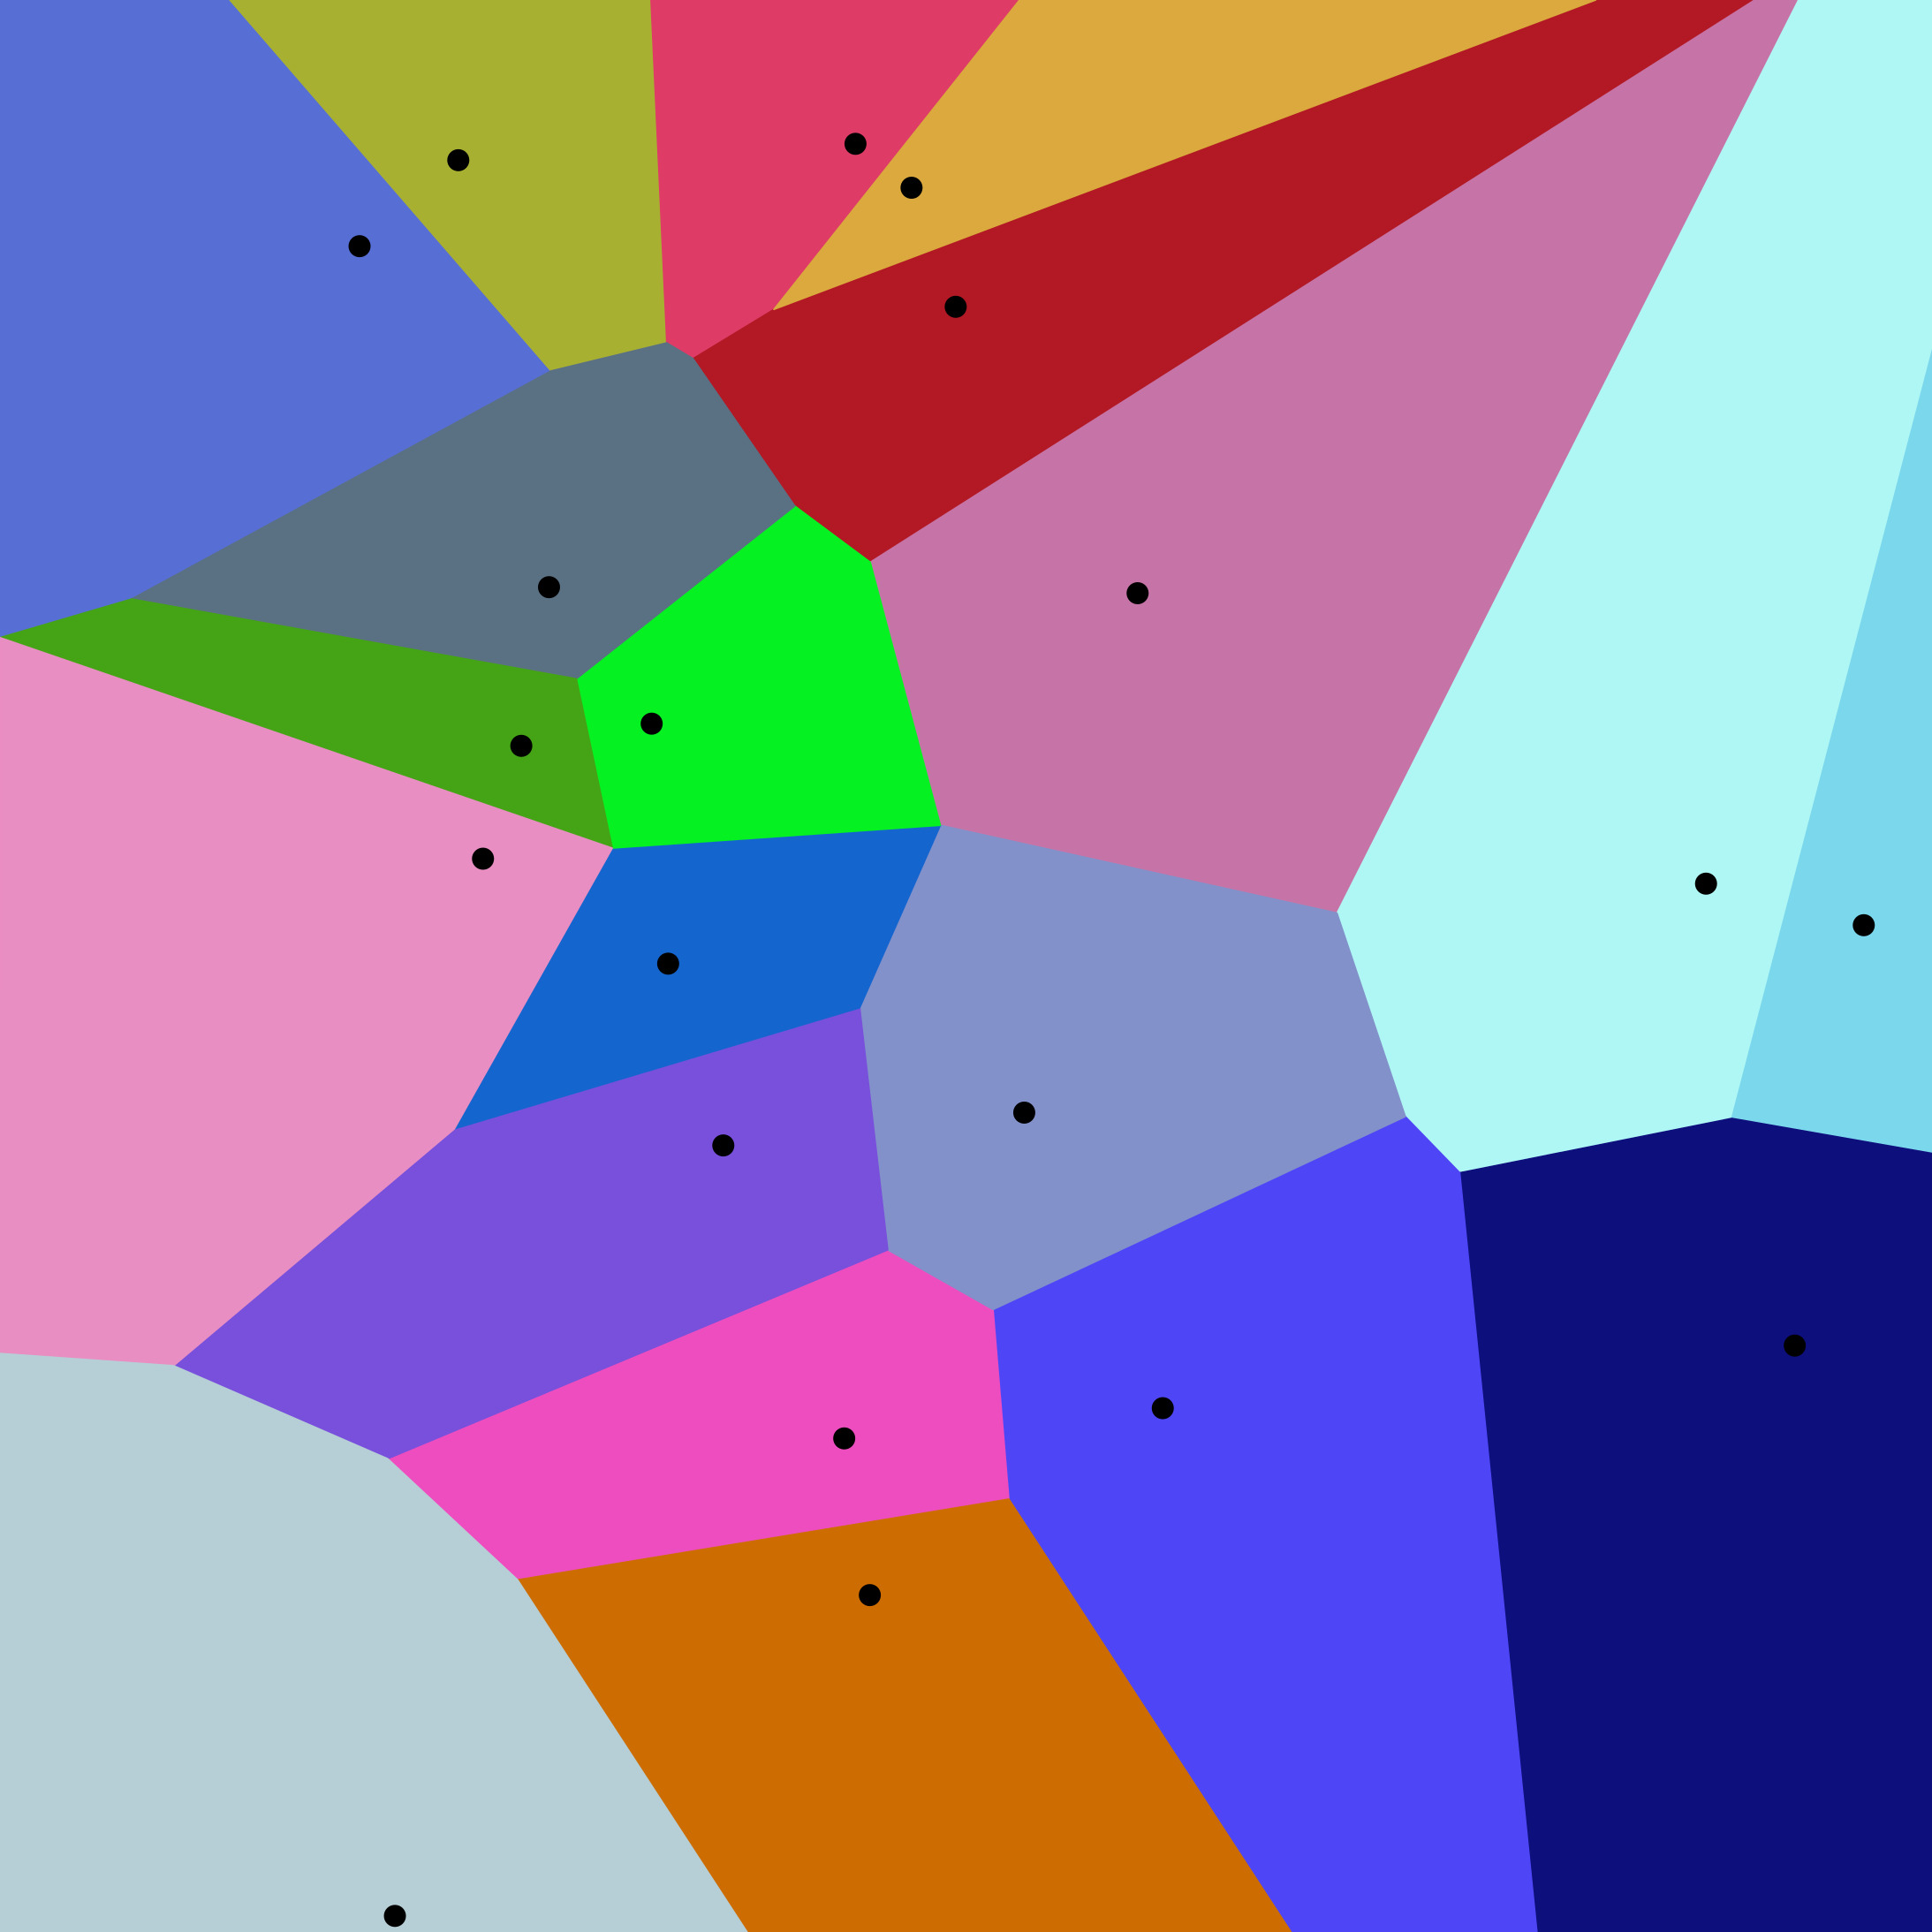
\includegraphics[width=0.48\textwidth, height=0.48\textwidth]{./fig/diagrams/Euclidean_Voronoi_diagram.jpg}
            \label{fig:voronoi_2d}
            }
            \subfloat[Euclidean Voronoi Diagram in \ac{3D}] {
            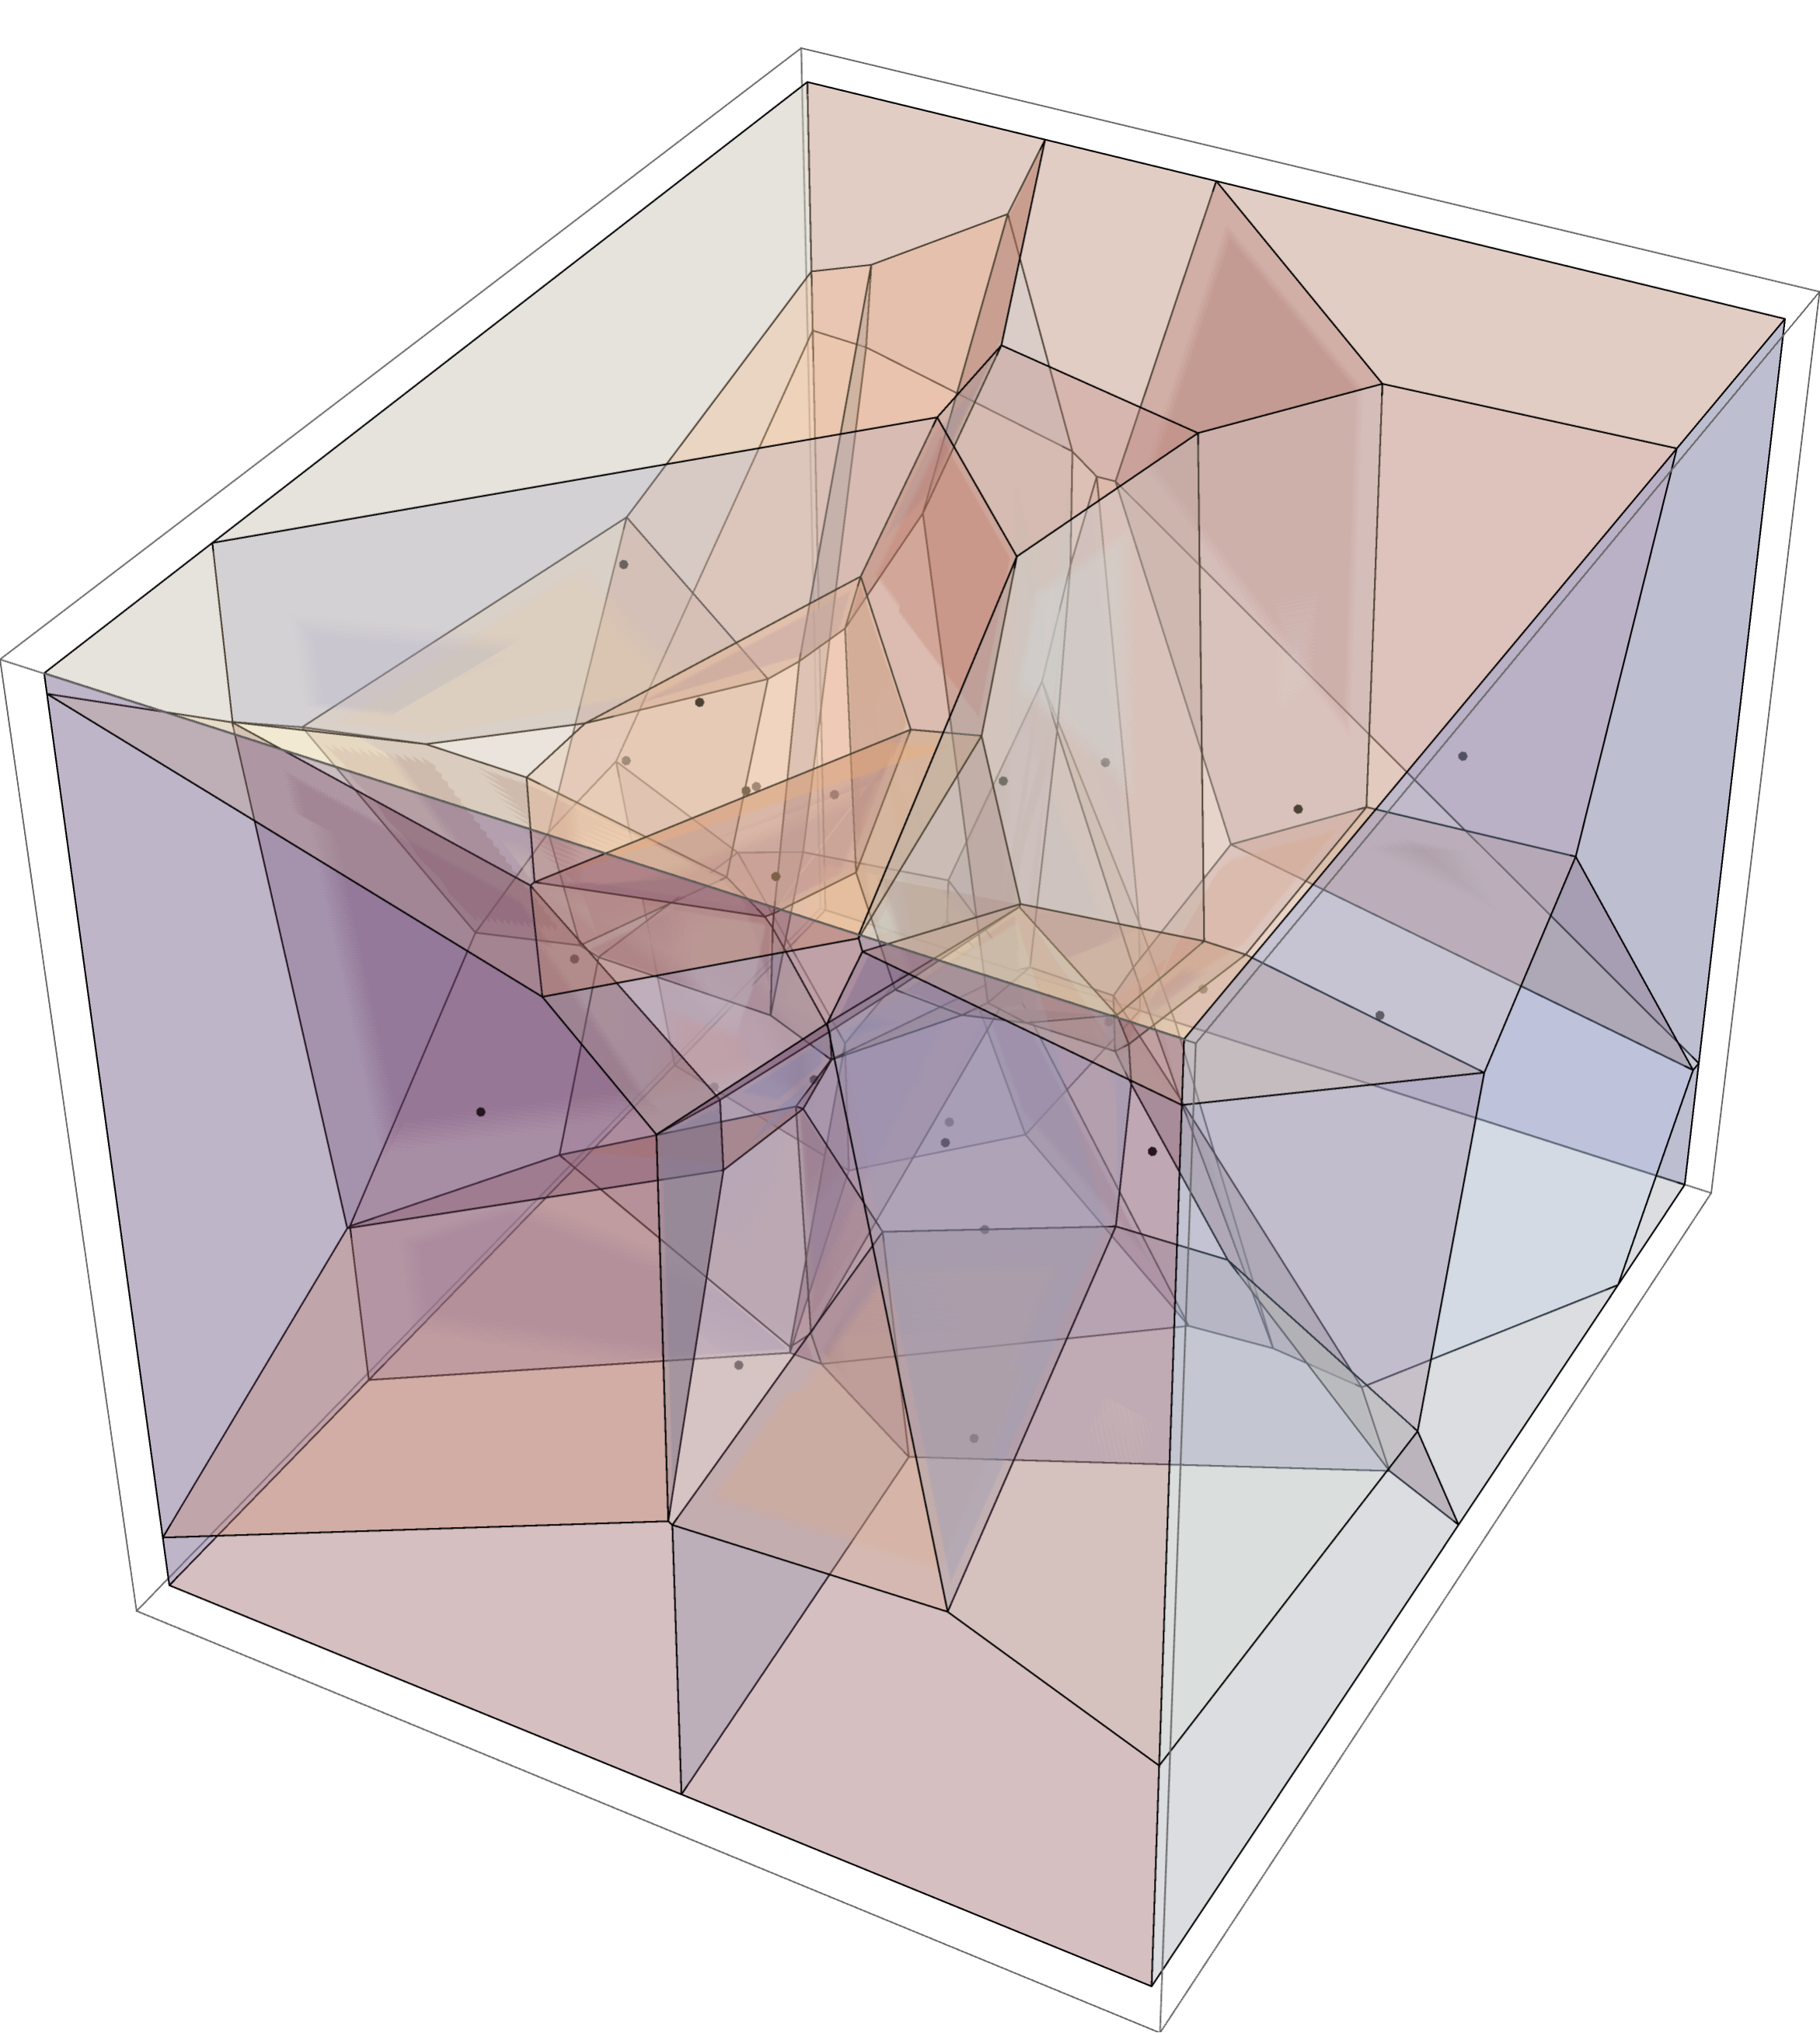
\includegraphics[width=0.48\textwidth, height=0.48\textwidth]{./fig/diagrams/Euclidian Voronoi diagram 3d.png}
            \label{fig:voronoi_3d}
            }
            \caption{
                (a) an example of 20 Voronoi cells in \ac{2D} \cite{Voronoi2d} (b) 25 Voronoi cells in \ac{3D} \cite{Voronoi3d}
            }
            \label{fig:voronoi_diagrams}
        \end{figure}
    
    \subsection{Additional Constraints and Modifications}
        To extend the approach to the \ac{3D} case, several adjustments are made.
        The weighting rule (\ref{eqn:beta_weighting}) remains unchanged. 
        However, in both the azimuth update rule (\ref{eqn:azimuth_2d}) and the azimuth reset rule (\ref{eqn:azimuth_reset_2d}), only the displacement of centroids projected onto the $xy$-plane is taken into account.
        The modified formulations for the \ac{3D} case are as follow:
        \begin{itemize}
            \item \textbf{Azimuth update rule \ac{3D}}
                \begin{equation}
                    \label{eqn:azimuth_3d}
                    \dot{\theta}_i = 
                    \begin{cases}
                        k  & \text{if } \theta < \frac{\pi}{2} \land \|\mathbf{c}_{\mathcal{A}_i} - \mathbf{c}_{\mathcal{S}_i}\|_{xy} > d_4 \land \|\mathbf{p}_i - \mathbf{c}_{\mathcal{A}_i}\|_{xy} > d_3 \\
                        -k & \text{if } \theta > 0 \land \neg (\|\mathbf{c}_{\mathcal{A}_i} - \mathbf{c}_{\mathcal{S}_i}\|_{xy} > d_4 \land \|\mathbf{p}_i - \mathbf{c}_{\mathcal{A}_i}\|_{xy} > d_3) \\
                        0  & \text{otherwise}
                    \end{cases}
                \end{equation}
            \item \textbf{Azimuth reset rule \ac{3D}}
                \begin{equation}
                    \label{eqn:azimuth_reset_3d}
                    \theta = 0 \quad \text{if } \theta = \frac{\pi}{2} \land \| \mathbf{p}_i - \mathbf{\overline{c}}_{\mathcal{A}_i} \|_{xy}    
                \end{equation}
        \end{itemize}

        The notation $\| \cdot \|_{xy}$ denotes the Euclidean norm computed in the $xy$-plane only, defined as:
        \begin{equation}
            \| \mathbf{p}_i - \mathbf{p}_j \|_{xy} = \sqrt{(x_i - x_j)^2 + (y_i - y_j)^2}
        \end{equation}



        Additionally, $Z_{clipping}$ is applied to each sensing cell $\mathcal{S}_i$, constraining it within the vertical limits defined by $\text{min}_z$ and $\text{max}_z$:

        \begin{equation}
            \mathcal{S}_i = \left\{\mathbf{q} \in \mathcal{Q} \mid \|\mathbf{q} - \mathbf{p}_i\| \leq r_{s,i}, \quad \text{min}_z \leq q_z \leq \text{max}_z \right\}
        \end{equation}

        where $\text{min}_z$ and $\text{max}_z$ define the vertical bounds within which the sensing region $\mathcal{S}_i$ is restricted. 
        This ensures that the agent cannot exceed these limits, as it follows the computed centroid \( \mathbf{c}_{V_i} \). 
        By constraining the sensing radius, the agent remains confined within the specified region, preventing it from moving outside the vertical interval $\text{min}_z$ to $\text{max}_z$.

        The destination rotation rule $Z_{rule}$ is introduced to enhance agents avoidance by rotating the computed destination $\mathbf{d}_i$ by an angle $\phi$.
        For vertical rotation angle $\phi$, the following condition is intorduced
        \begin{equation}
            \label{eqn:phi_condition}
            \Omega = \|\mathbf{c}_{\mathcal{A}_i} - \mathbf{c}_{\mathcal{S}_i}\|_z < d_6 \land \|\mathbf{p}_i - \mathbf{c}_{\mathcal{A}_i}\|_z \lor 
            | \|\mathbf{p}_i - \mathbf{c}_{\mathcal{S}_i}\|_{xy} - \|\mathbf{p}_i - \mathbf{c}_{\mathcal{A}_i}\|_{xy} | > d_7
        \end{equation}
        This condition has two main parts, combined by a logical or. The first part evaluates the vertical displacement of the centroid of the partitioned cell $\mathbf{c}_{\mathcal{A}_i}$ from the centroid of the sensing cell $\mathbf{c}_{\mathcal{S}_i}$ and the
        displacement of the agents position $\mathbf{p}_i$ from  $\mathbf{c}_{\mathcal{A}_i}$.
        The second part considers the difference in the horizontal plane between the agent's position and the centroids $\mathbf{c}_{\mathcal{A}_i}$, $\mathbf{c}_{\mathcal{S}_i}$.

        To improve agent distriution in the vertical dimension, a directional influence on vertical exploration is introduced. 
        Given that each agent's position $\mathbf{p}_i$ and final goal $\mathbf{g}_i$, are known, this directional influence can be included into the update rule for $\phi_i$.

        First, the global heading angle, $\theta_{goal}$, towards the goal is calculated: 
        \begin{equation}
            \theta_{goal} = \text{atan2}(g_{i,y} - p_{i,y}, g_{i,x} - p_{i,x})
        \end{equation}
        where $\mathbf{g}_{i, x}$, $\mathbf{g}_{i, y}$ represent the x and y coordinates of the goal, and $\mathbf{p}_{i, x}$, $\mathbf{p}_{i, y}$ represent the x and y coordinates of the agent.
        The resulting angle is in the range $[-\pi, \pi]$.
        Next, the heading angle is linearly mapped to a direction influence $D_{influence}$ value in the range [-1, 1]:
        \begin{equation}
            D_{influence} = \frac{\theta_{goal}}{\pi}
        \end{equation}
        This mapping ensures that agents traveling directly northward (from South to North) have a directional influence close to one, that will promote upward vertical exploration. 
        Similarly, agents traveling southward have a direction influence close to -1, promoting downward exploration. 
        Agents moving primarily eastward or westward have a directional influence close to 0, resulting in minimal vertical exploration.
        This strategy encourages a more uniform distribution of agents throughout the \ac{3D} space. 

        To determine the adjustment to the agent's vertical orientation, the directional influence $D_{influence}$ is combined with the relative vertical displacement of the agent and $\mathbf{c}_{\mathcal{S}_i}$
        Weighted average is used to combine them: 
        \begin{equation}
            \label{eqn:combined_influace}
            C_{influence} = \frac{w_1 \cdot (\mathbf{c}_{\mathcal{S}_i,z} - \mathbf{p}_{i,z}) + w_2 \cdot D_{influence}}{w_1 + w_2}
        \end{equation} 
        where $w_1$ $w_2$ are weighting factors. The resulting combined influence $C_{influence}$ is then used to update the agent's rotation of it's destination $\mathbf{d}_i$ by $\phi_i$.

        Based on condition \eqref{eqn:phi_condition} and \eqref{eqn:combined_influace} update rule for $\phi_i$ can be constructed as follows:
        \begin{equation}
            \label{eqn:phi_update}
            \dot{\phi}_i = 
            \begin{cases}
                k  & \text{if } \phi_i < \frac{\pi}{4} > \land C_{influence} > 0 \land \Omega \\
                0  & \text{if } \phi_i > \frac{\pi}{4} > \land C_{influence} > 0 \land \Omega \\
                -k & \text{if } \phi_i > -\frac{\pi}{4} > \land C_{influence} \leq 0 \land \Omega \\
                0  & \text{if } \phi_i < -\frac{\pi}{4} > \land C_{influence} \leq 0 \land \Omega \\
                -k & \text{if } \phi_i > 0 \land \neg \Omega \\
                k  & \text{if } \phi_i < 0 \land \neg \Omega \\
                0  & \text{otherwise}
            \end{cases}
        \end{equation}
        where the first four cases control the rotation of the agent's destination $\mathbf{d}_i$ and the final three cases handle the smooth convergence of $\phi_i$ back to 0, when the condition $\Omega$ is not met. 

        After the application of the rules for $\theta_i$ and $\phi_i$, the agent's destination is updated as:
        \begin{equation}
            \label{eqn:destination_update}
            \mathbf{d}_i =
            \begin{pmatrix}
                p_{i,x} +  \|\mathbf{p}_i - \mathbf{g}_i\| \cdot \sin(\phi_{\mathbf{g}_i} + \phi_i) \cdot \cos(\theta_{\mathbf{g}_i} - \theta_i) \\
                p_{i,y} + \|\mathbf{p}_i - \mathbf{g}_i\| \cdot \sin(\phi_{\mathbf{g}_i} + \phi_i) \cdot \sin(\theta_{\mathbf{g}_i} - \theta_i) \\
                p_{i,z} + \|\mathbf{p}_i - \mathbf{g}_i\| \cdot \cos(\phi_{\mathbf{g}_i} + \phi_i)
            \end{pmatrix}
        \end{equation}

        where $\phi_{\mathbf{g}_i} = \arccos(\frac{\mathbf{g}_{i,z} - \mathbf{p}_{i,z}}{\|\mathbf{p}_i - \mathbf{g}_i\|})$ is the polar angle from z-axis to the goal, 
        $\theta_{\mathbf{g}_i} = atan2( \mathbf{g}_{i,y} - \mathbf{p}_{i,y}, \mathbf{g}_{i,x} - \mathbf{p}_{i,x})$ is the azimuthal angle in the xy-plane to the goal.
    
    \subsection{Algorithm Walkthrough}
        At each iteration, the proposed algorithm performs a sequence of actions to control agent movement. 
        These actions can be summarized as follows:
        \begin{enumerate}
            \item \textbf{Cell Generation:} \\
                For each agent, two cells are generated: a partitioned cell, denoted as $\mathcal{A}$ and a sensing cell, denoted as $\mathcal{S}$.
            \item \textbf{Centroid Computation:}
                \begin{itemize}
                    \item The centroid of cell $\mathcal{A}$, $c_{\mathcal{A}}$ is computed using a weighted function that considers both the agent's goal position, $\mathbf{g}_i$, and its current destination, $\mathbf{d}_i$.
                    \item The centroid of cell $\mathcal{S}$, $c_{\mathcal{S}}$ is computed using a weighted function that considers only the agent's current destination, $\mathbf{d}_i$.
                \end{itemize}
            \item \textbf{Rule Application and Destination Update:} \\
                A set of rules is applied to: 
                \begin{itemize}
                    \item Adjust weighting function usied in the centroid computations \eqref{eqn:beta_weighting}.
                    \item Rules to update $\theta_i$ \eqref{eqn:azimuth_3d} and $\phi_i$ \eqref{eqn:phi_update} are applied.
                    \item Update the agent's destination $\mathbf{d}_i$ \eqref{eqn:destination_update}.
                \end{itemize}
            \item \textbf{Agent movement} \\
                Finally, the agent is directed towards a centroid location $c_{\mathcal{A}}$.
        \end{enumerate}
        This process is repeated until all agents reach their goals.

        

\section{Simulation and Results Analysis}

    \subsection{Computational Implementation Details}
        The continuous algorithm presented in the previous section can be easily discretized for implementation in a computational enviroment.
        Instead of continuous sets, the cells $\mathcal{A}$ and $\mathcal{S}$ are aproximated using a set of discrete points.   
        Discrete points are partitioned out when definition \eqref{eq:voronoi_cell_account_encum} is not met.
        \begin{figure}[H]
            \centering
            \subfloat[Example of discretized cells ($\mathcal{A} = \mathcal{S}$)] {
            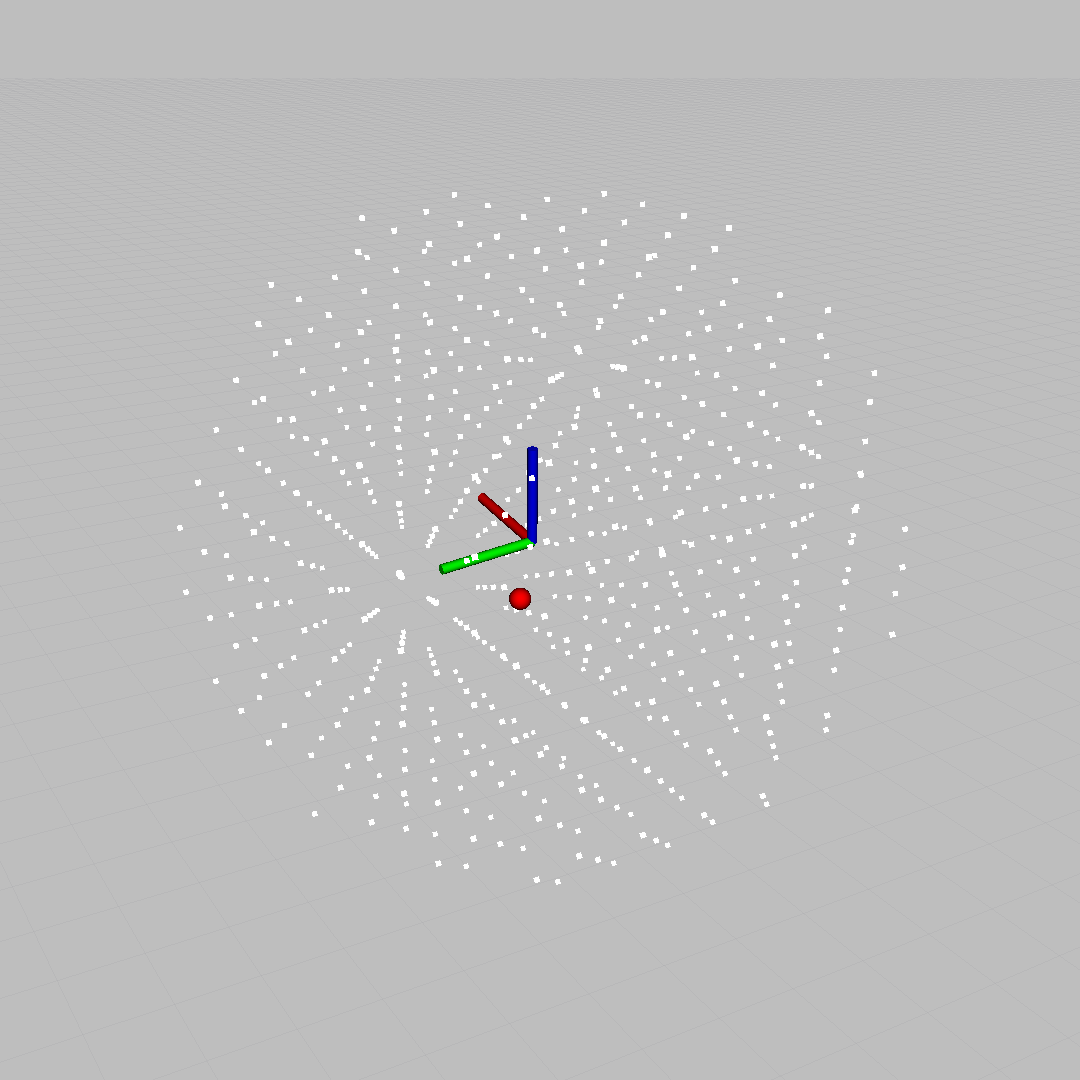
\includegraphics[width=0.48\textwidth, height=0.48\textwidth]{./fig/rviz/cs_equal_ca.png}
            \label{fig:rviz_cs_eq_ca}
            }
            \subfloat[Example of a partitioned cell $\mathcal{A}$] {
            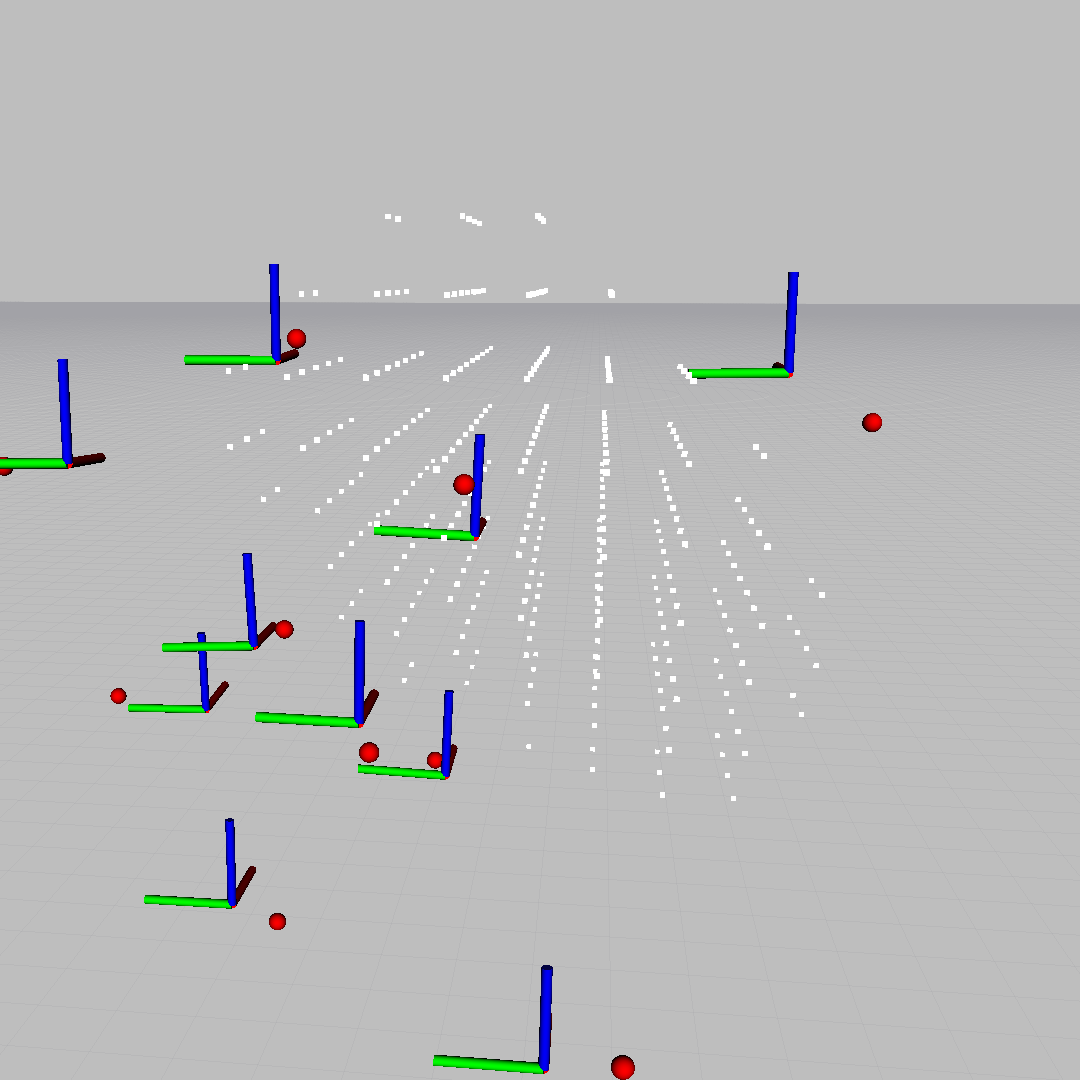
\includegraphics[width=0.48\textwidth, height=0.48\textwidth]{./fig/rviz/ca_partitioned.png}
            \label{fig:rviz_ca_partitioned}
            }
            \caption{
                Discrete approximation of Voronoi cells, with centroid $c_{\mathcal{A}}$ shown as a red dot.(a) Example where the partitioned cell $\mathcal{A}$ and the sensing cell $\mathcal{S}$ are the same. (b) Example where the partitioned cell $\mathcal{A}$ is partitioned by other \ac{UAV}s.
            }
            \label{fig:rviz_cells}
        \end{figure}
        
    \subsection{Simulation Enviroment}
        In this simulation, the term 'agent' refers to the \ac{UAV}, which were simulated using the framework provided by \ac{MRS} \cite{mrs_uav_system}.
        Each \ac{UAV} obtains its global ground truth position from the ROS simulator.
        The positions of neighboring \ac{UAV}s were estimated using simulated blinking ultraviolet markers, following the method described in \cite{uvdd1} and \cite{uvdar_package}.
        The following constraints are relevant for each \ac{UAV}:
        \begin{table}[h]
            \centering
            \renewcommand{\arraystretch}{1.1}
            \begin{tabular}{|l|c|}
                \hline
                \textbf{Parameter} & \textbf{Value} \\ \hline
                    Maximal horizontal velocity [\SI{}{\meter\per\second}] & 4.0 \\ \hline
                    Horizontal acceleration [\SI{}{\meter\per\second\squared}] & 2.0 \\ \hline
                    Maximal ascending velocity [\SI{}{\meter\per\second}] & 2.0 \\ \hline
                    Vertical ascending acceleration [\SI{}{\meter\per\second\squared}] & 1.0 \\ \hline
                    Maximal descending velocity [\SI{}{\meter\per\second}] & 2.0 \\ \hline
                    Vertical descending acceleration [\SI{}{\meter\per\second\squared}] & 1.0 \\ \hline
                \end{tabular}
                \caption{Motion constraints of the \ac{UAV}.}
            \label{tab:uav_constraints}
        \end{table}
        
    \subsection{Simulation Scenarios}
        To evaluate the safety and performance of the \ac{UAV}s during interactions, a series of experiments was conducted. 
        Experiments were performed primarily using circular formations, with \ac{UAV} counts of N = 5, 10, and 15. 
        Each of these circular formation experiments was repeated 10 times.
        Additionally, to extend the analysis to \ac{3D} and assess the algorithm's performance, a set of spherical formation experiments was conducted with N = 10, also repeated 10 times.
        After each \ac{UAV} was flown from the ground to its starting position, the \ac{RBL} algorithm was activated.    

        These formations provide a controlled enviroment compared to random initial position and goal locations. 
        In both circular and spherical formations, the \ac{UAV}s were evenly distributed along the circle or the surface of the sphere, with the goal position located on the opposite side.
        The radius of both circle and the sphere was set to 5 meters.
        
        The following metrics were measured across the 10 repetitions of each experiment, along with their standard deviations: success rate \( SR \ [\%] \), average trajectory length \( \overline{L} \ [\mathrm{m}] \), 
        average time to reach the goal \( \overline{t} \ [\mathrm{s}] \), average of the maximal time for \ac{UAV} to reach the goal \( \overline{t}_{\text{max}} \ [\mathrm{s}] \), and average velocity \( \overline{v} \ [\mathrm{m/s}] \).

        The specific values of the parameters used in the experiments are summarized in following table \ref{tab:experiment_parameters}:
        \begin{table}[H]
            \centering
            \caption{Parameters Used in Experiments}
            \begin{tabular}{|l|l|}
                \hline
                Parameter & Value \\
                \hline
                \hline
                Sensing radius ($r_s$) & 3.5 m \\ \hline
                Update rate & 10 Hz \\ \hline
                Encumbrance & 0.5 m \\ \hline
                $d_1 = d_3 = d_5$ & 0.5 m \\ \hline
                $d_2 = d_4 = d_6$ & 1.0 m \\ \hline
                $d_7$ & 0.2  \\ \hline
                $\beta_i^D$ & 1.5  \\ \hline
                $\eta$ & 0.9  \\ \hline
                $min_z$ & 1.0 m \\ \hline
                $max_z$ & 10.0 m \\ \hline
                $w_1$ & 0.7 \\ \hline
                $w_2$ & 0.3 \\ \hline

            \end{tabular}
            \label{tab:experiment_parameters}
        \end{table}

    \subsection{Experimental Results}
        \begin{itemize}
            \item \textbf{$N = 5$ Circular Formation:}
                \begin{table}[H]
                    \centering
                    \renewcommand{\arraystretch}{1.2}
                    \begin{tabular}{|l|c|c|c|c|c|}
                    \hline
                                                & \( SR \ [\%] \) & \( \overline{L} \ [\mathrm{m}] \) & \( \overline{t} \ [\mathrm{s}] \) & \( \overline{t}_{\text{max}} \ [\mathrm{s}] \) & \( \overline{v} \ [\mathrm{m/s}] \)     \\ \hline
                    RBL \ac{2D}                      & 100.00          & 21.06 $\pm$ 0.10                  & 25.15 $\pm$ 0.21                  & 25.15 $\pm$ 0.19                               & 0.83 $\pm$ 0.01                         \\ \hline
                    RBL \ac{3D}                      & 100.00          & 20.77 $\pm$ 0.29                  & 26.04 $\pm$ 0.51                  & 26.79 $\pm$ 0.27                               & 0.79 $\pm$ 0.02                         \\ \hline
                    RBL \ac{3D}\(_{\text{clipped}}\) & 100.00          & 20.60 $\pm$ 0.24                  & 26.73 $\pm$ 0.47                  & 27.39 $\pm$ 0.28                               & 0.77 $\pm$ 0.02                         \\ \hline
                    RBL \ac{3D}\(_z\)                & 100.00          & 20.97 $\pm$ 0.52                  & 25.54 $\pm$ 0.97                  & 26.72 $\pm$ 0.60                               & 0.81 $\pm$ 0.03                         \\ \hline
                    \end{tabular}
                \end{table}
            \item \textbf{$N = 10$ Circular Formation:}
                \begin{table}[H]
                    \centering
                    \renewcommand{\arraystretch}{1.2}
                    \begin{tabular}{|l|c|c|c|c|c|}
                    \hline
                                                & \( SR \ [\%] \) & \( \overline{L} \ [\mathrm{m}] \) & \( \overline{t} \ [\mathrm{s}] \) & \( \overline{t}_{\text{max}} \ [\mathrm{s}] \) & \( \overline{v} \ [\mathrm{m/s}] \)     \\ \hline
                    RBL \ac{2D}                      & 100.00          & 22.95 $\pm$ 1.64                  & 30.79 $\pm$ 2.28                  & 34.73 $\pm$ 0.77                               & 0.74 $\pm$ 0.07                         \\ \hline
                    RBL \ac{3D}                      & 100.00          & 22.22 $\pm$ 0.89                  & 30.05 $\pm$ 2.61                  & 34.39 $\pm$ 4.19                               & 0.73 $\pm$ 0.05                         \\ \hline
                    RBL \ac{3D}\(_{\text{clipped}}\) & 100.00          & 22.31 $\pm$ 0.69                  & 30.22 $\pm$ 1.83                  & 33.22 $\pm$ 0.93                               & 0.73 $\pm$ 0.04                         \\ \hline
                    RBL \ac{3D}\(_z\)                & 100.00          & 22.38 $\pm$ 0.88                  & 28.80 $\pm$ 2.30                  & 32.35 $\pm$ 1.25                               & 0.77 $\pm$ 0.05                         \\ \hline
                    \end{tabular}
                \end{table}
            \item \textbf{$N = 15$ Circular Formation:}
                \begin{table}[H]
                    \centering
                    \renewcommand{\arraystretch}{1.2}
                    \begin{tabular}{|l|c|c|c|c|c|}
                    \hline
                                                & \( SR \ [\%] \) & \( \overline{L} \ [\mathrm{m}] \) & \( \overline{t} \ [\mathrm{s}] \) & \( \overline{t}_{\text{max}} \ [\mathrm{s}] \) & \( \overline{v} \ [\mathrm{m/s}] \)     \\ \hline
                    RBL \ac{2D}                      & 100.00          & 23.56 $\pm$ 1.75                  & 33.89 $\pm$ 2.48                  & 38.75 $\pm$ 1.45                               & 0.69 $\pm$ 0.06                         \\ \hline
                    RBL \ac{3D}                      & 100.00          & 22.36 $\pm$ 0.97                  & 30.65 $\pm$ 3.07                  & 35.77 $\pm$ 3.72                               & 0.72 $\pm$ 0.07                         \\ \hline
                    RBL \ac{3D}\(_{\text{clipped}}\) & 100.00          & 22.32 $\pm$ 0.81                  & 30.69 $\pm$ 2.61                  & 34.50 $\pm$ 0.47                               & 0.72 $\pm$ 0.06                         \\ \hline
                    RBL \ac{3D}\(_z\)                & 100.00          & 22.64 $\pm$ 0.95                  & 29.67 $\pm$ 2.54                  & 34.27 $\pm$ 0.88                               & 0.76 $\pm$ 0.06                         \\ \hline
                    \end{tabular}
                \end{table}
            \item \textbf{$N = 10$ Spherical Formation:}
                \begin{table}[H]
                    \centering
                    \renewcommand{\arraystretch}{1.2}
                    \begin{tabular}{|l|c|c|c|c|c|}
                    \hline
                                                & \( SR \ [\%] \) & \( \overline{L} \ [\mathrm{m}] \) & \( \overline{t} \ [\mathrm{s}] \) & \( \overline{t}_{\text{max}} \ [\mathrm{s}] \) & \( \overline{v} \ [\mathrm{m/s}] \)     \\ \hline
                    RBL \ac{3D}                      & 100.00          & 14.32 $\pm$ 1.52                  & 27.76 $\pm$ 3.06                  & 32.48 $\pm$ 2.26                               & 0.51 $\pm$ 0.05                         \\ \hline
                    RBL \ac{3D}\(_z\)                & 100.00          & 14.06 $\pm$ 0.97                  & 27.17 $\pm$ 2.66                  & 31.86 $\pm$ 1.24                               & 0.55 $\pm$ 0.06                         \\ \hline
                    \end{tabular}
                \end{table}
        \end{itemize}

        The figure below visualizes the  \ac{UAV}  trajectories, showing the effect of the applied simulation rules.
        \begin{figure}[H]
            \centering
            \subfloat[Trajectories of \ac{UAV}s using 2D \ac{RBL}, $N=10$] {
                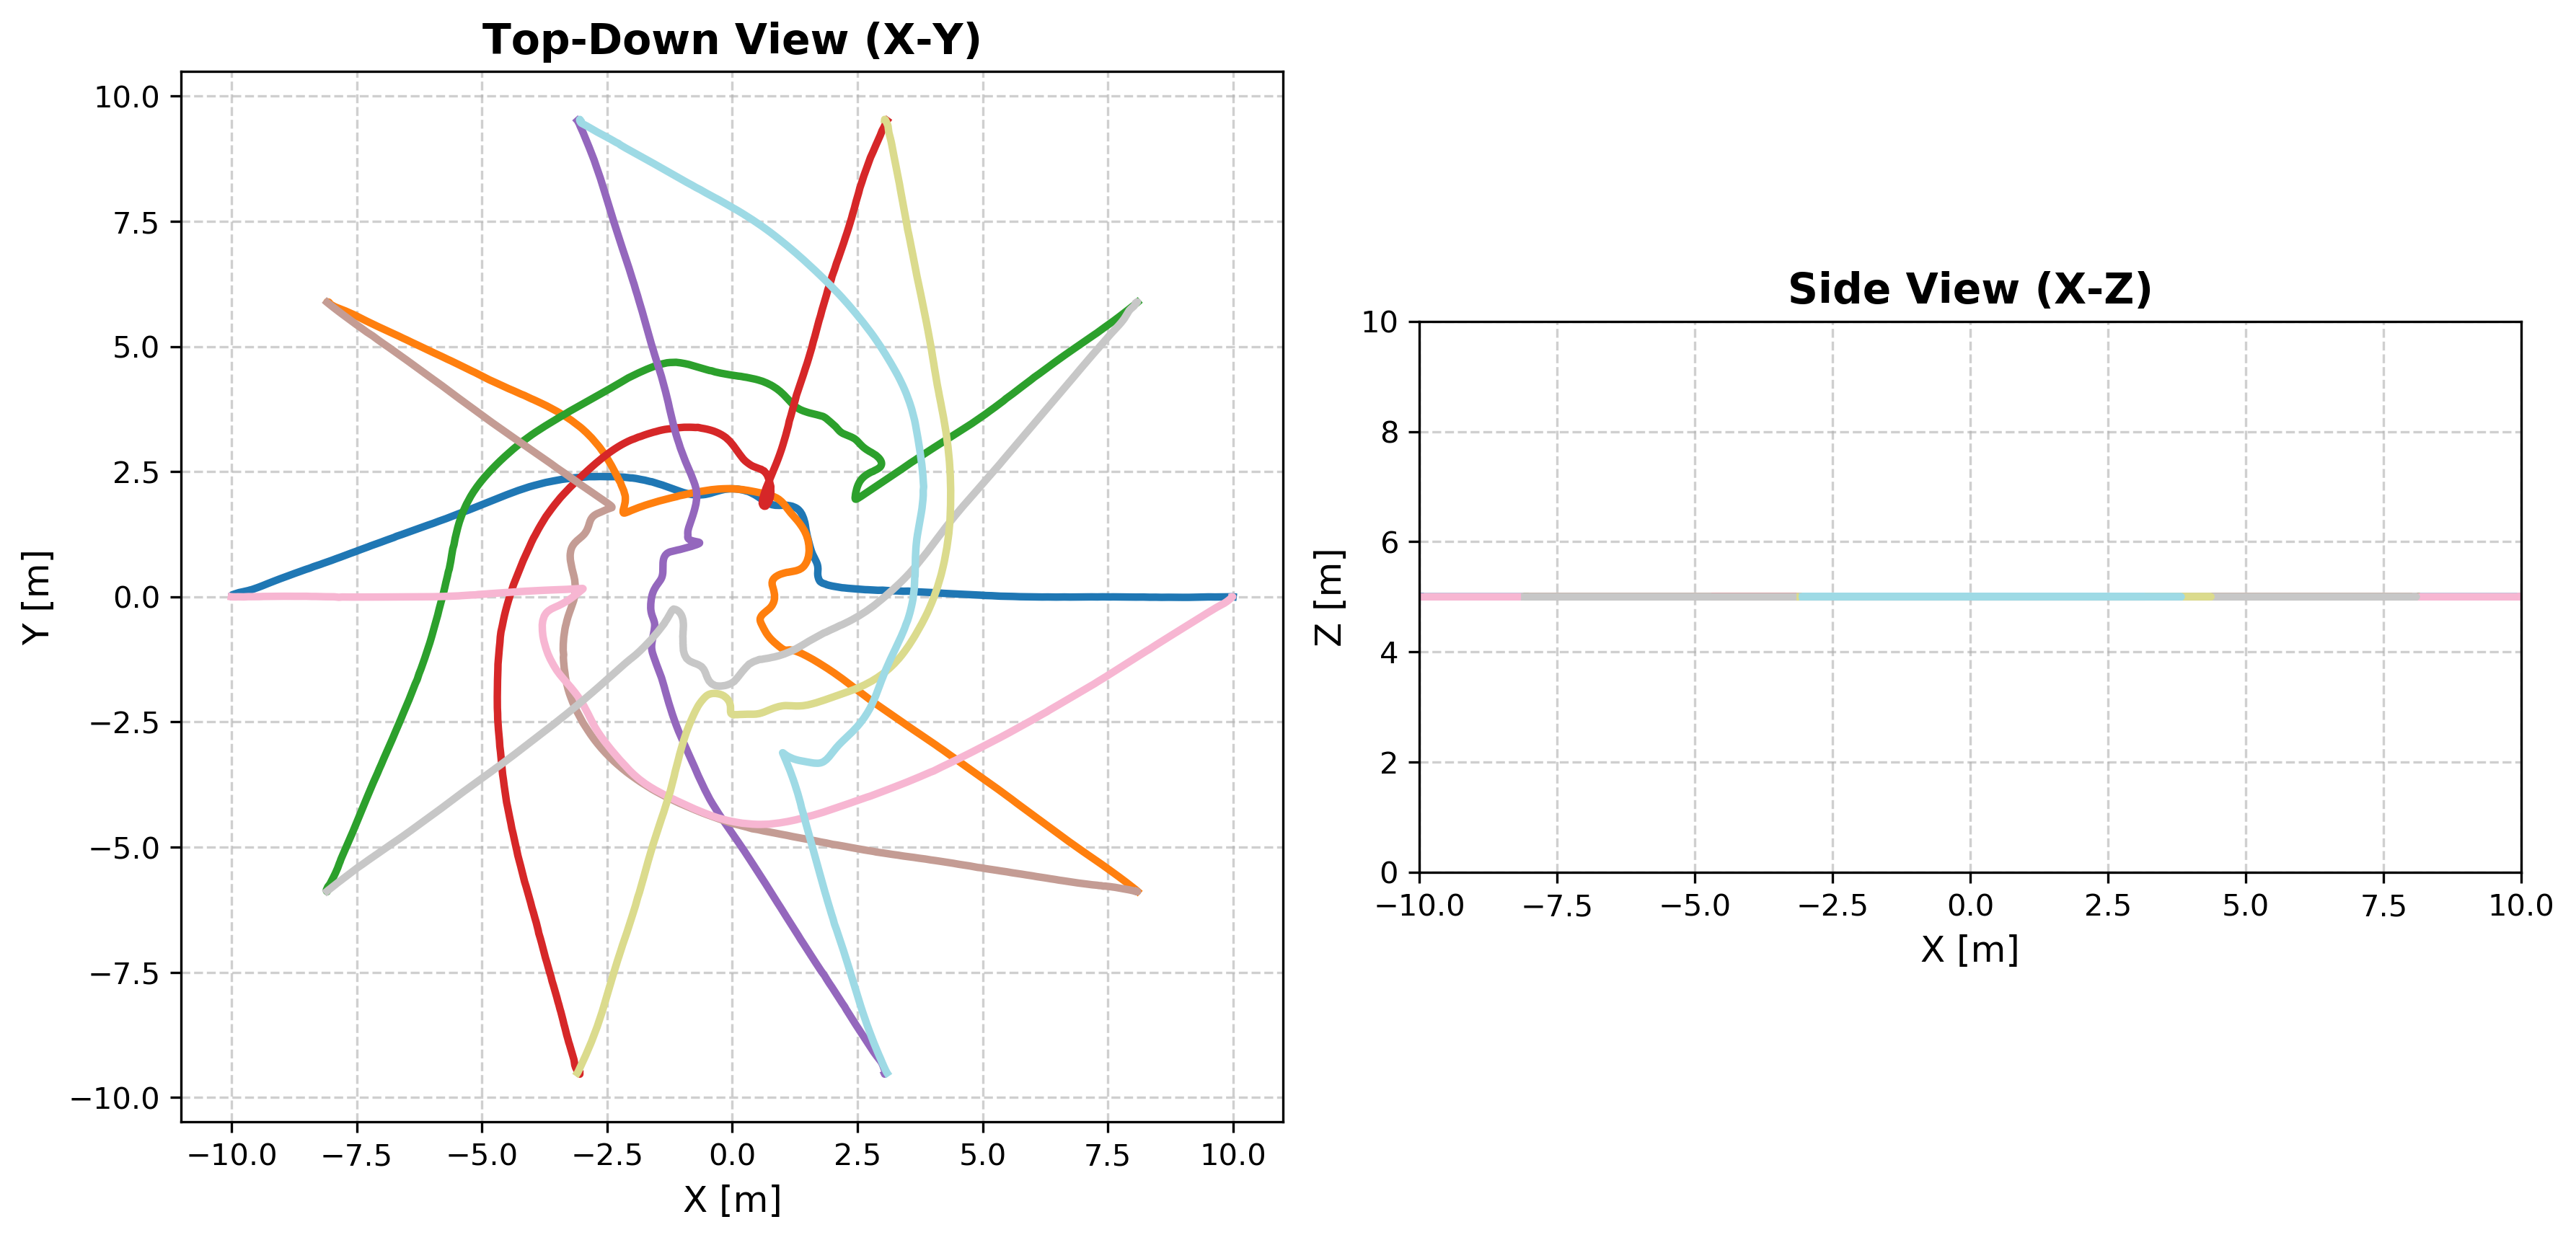
\includegraphics[width=0.48\textwidth, height=0.24\textwidth]{./fig/plots/n_10_circle_2d.png}
                \label{fig:n_10_circle_2d}
            }
            \subfloat[Trajectories of \ac{UAV}s using \ac{3D} \ac{RBL}, $N=10$] {
                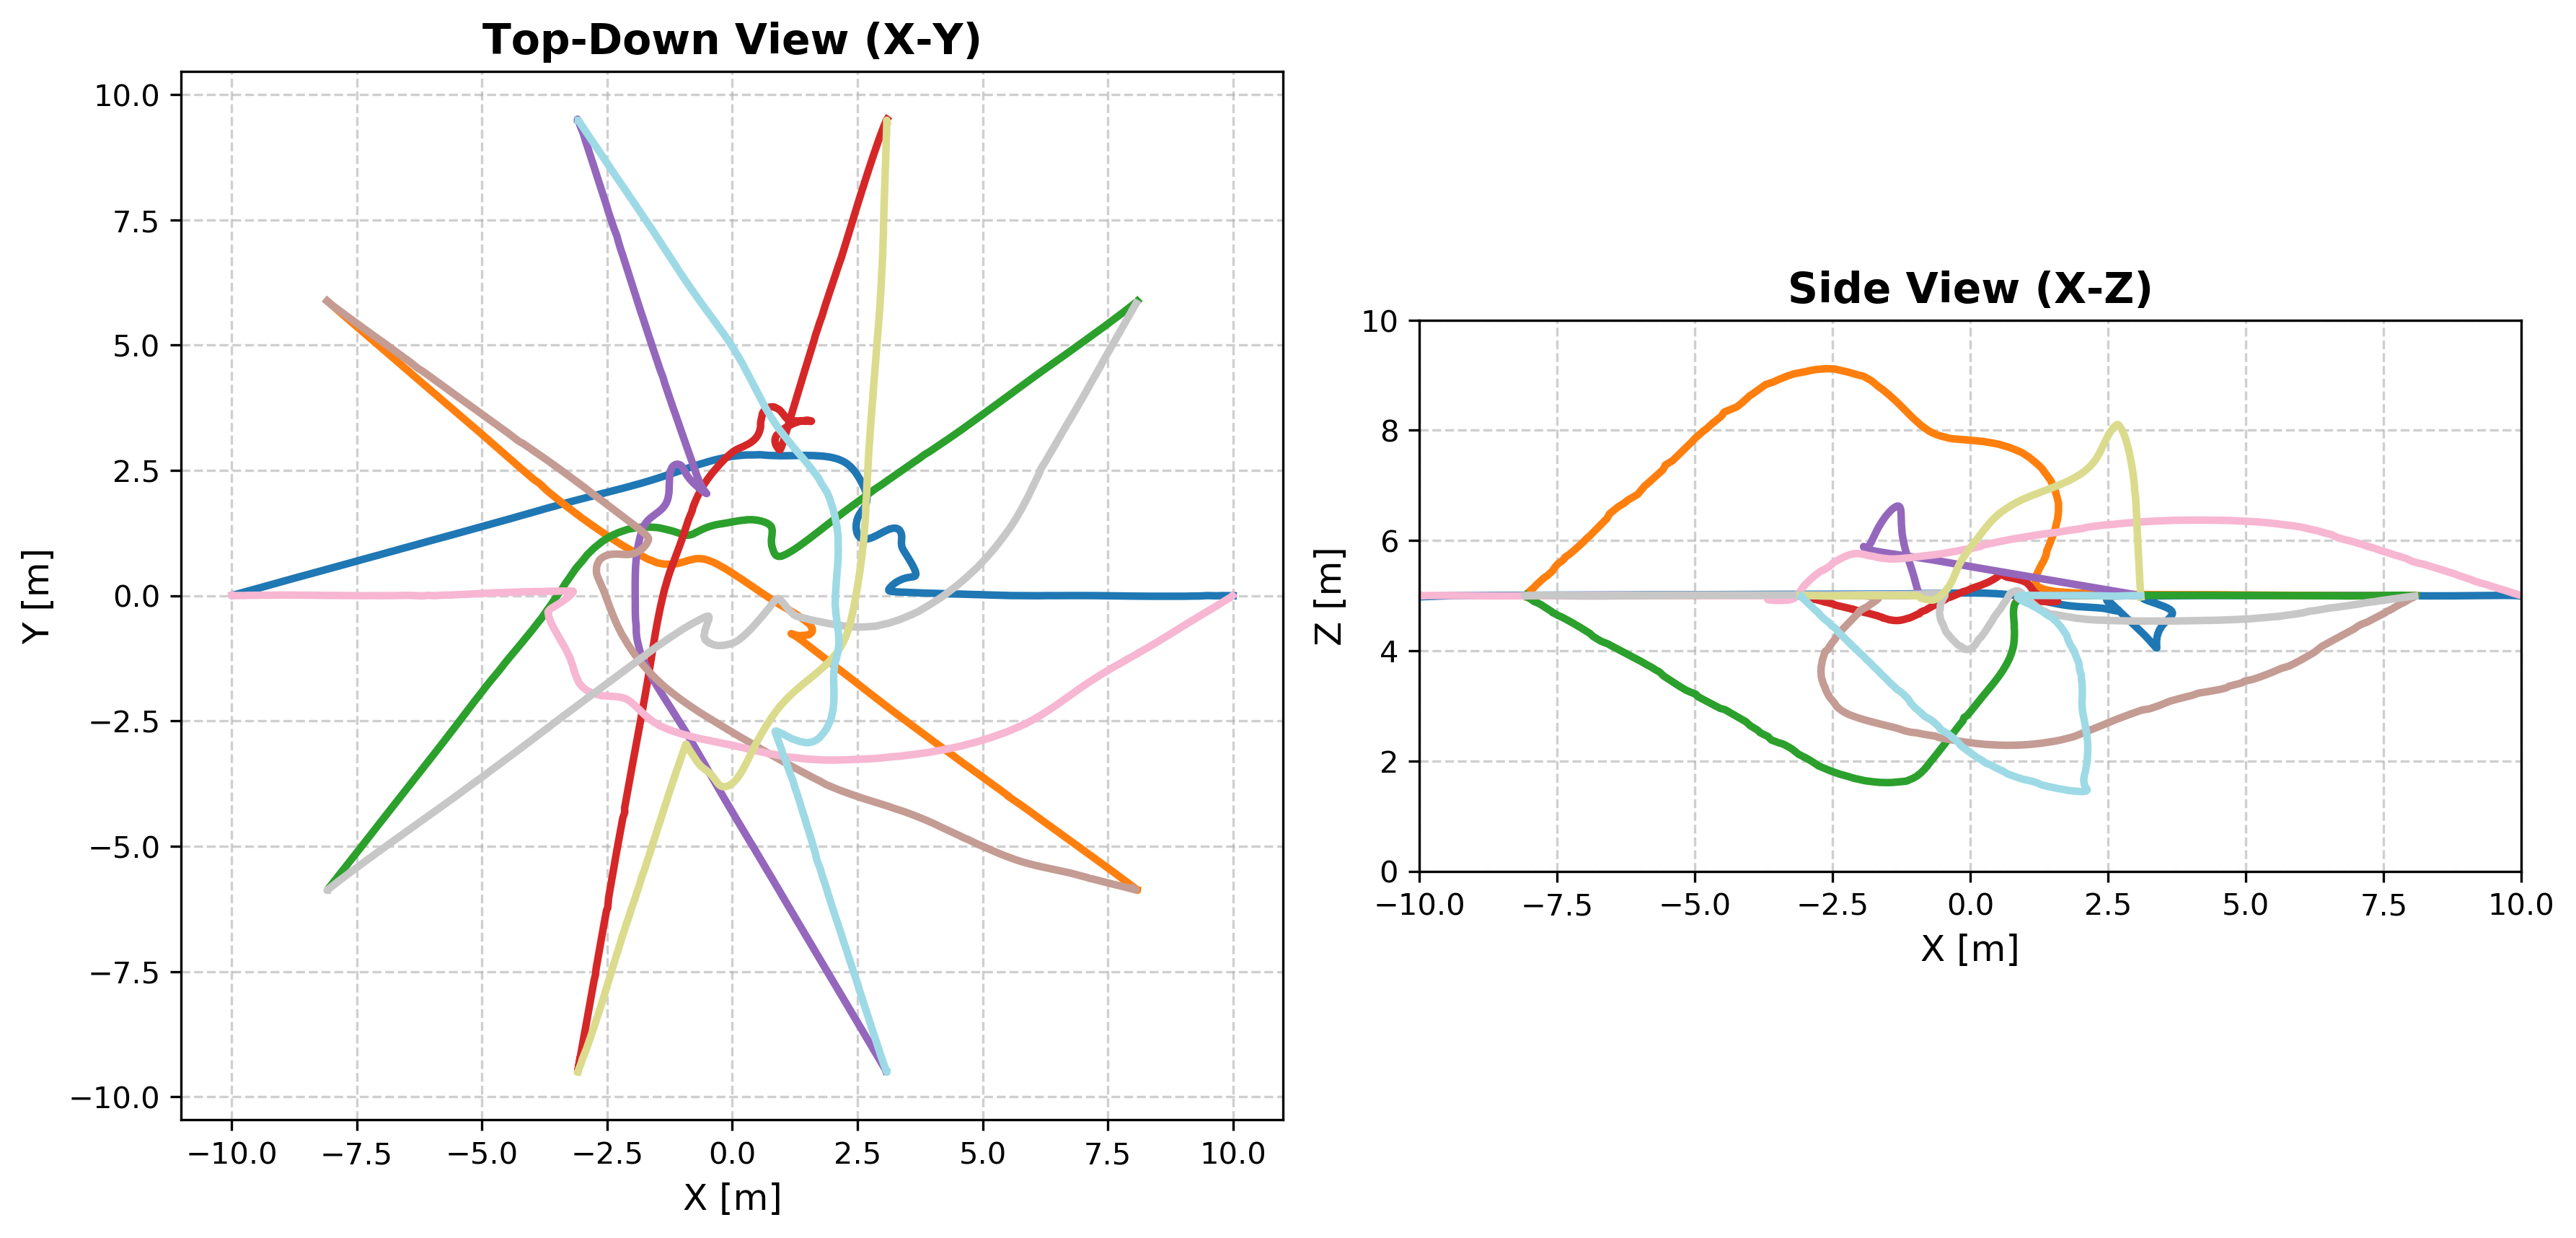
\includegraphics[width=0.48\textwidth, height=0.24\textwidth]{./fig/plots/n_10_circle_3d.png}
                \label{fig:n_10_circle_3d}
            }
            \par\medskip
            \subfloat[Trajectories of \ac{UAV}s using \ac{3D} \ac{RBL} and $Z_{clipping}$, $N=10$] {
                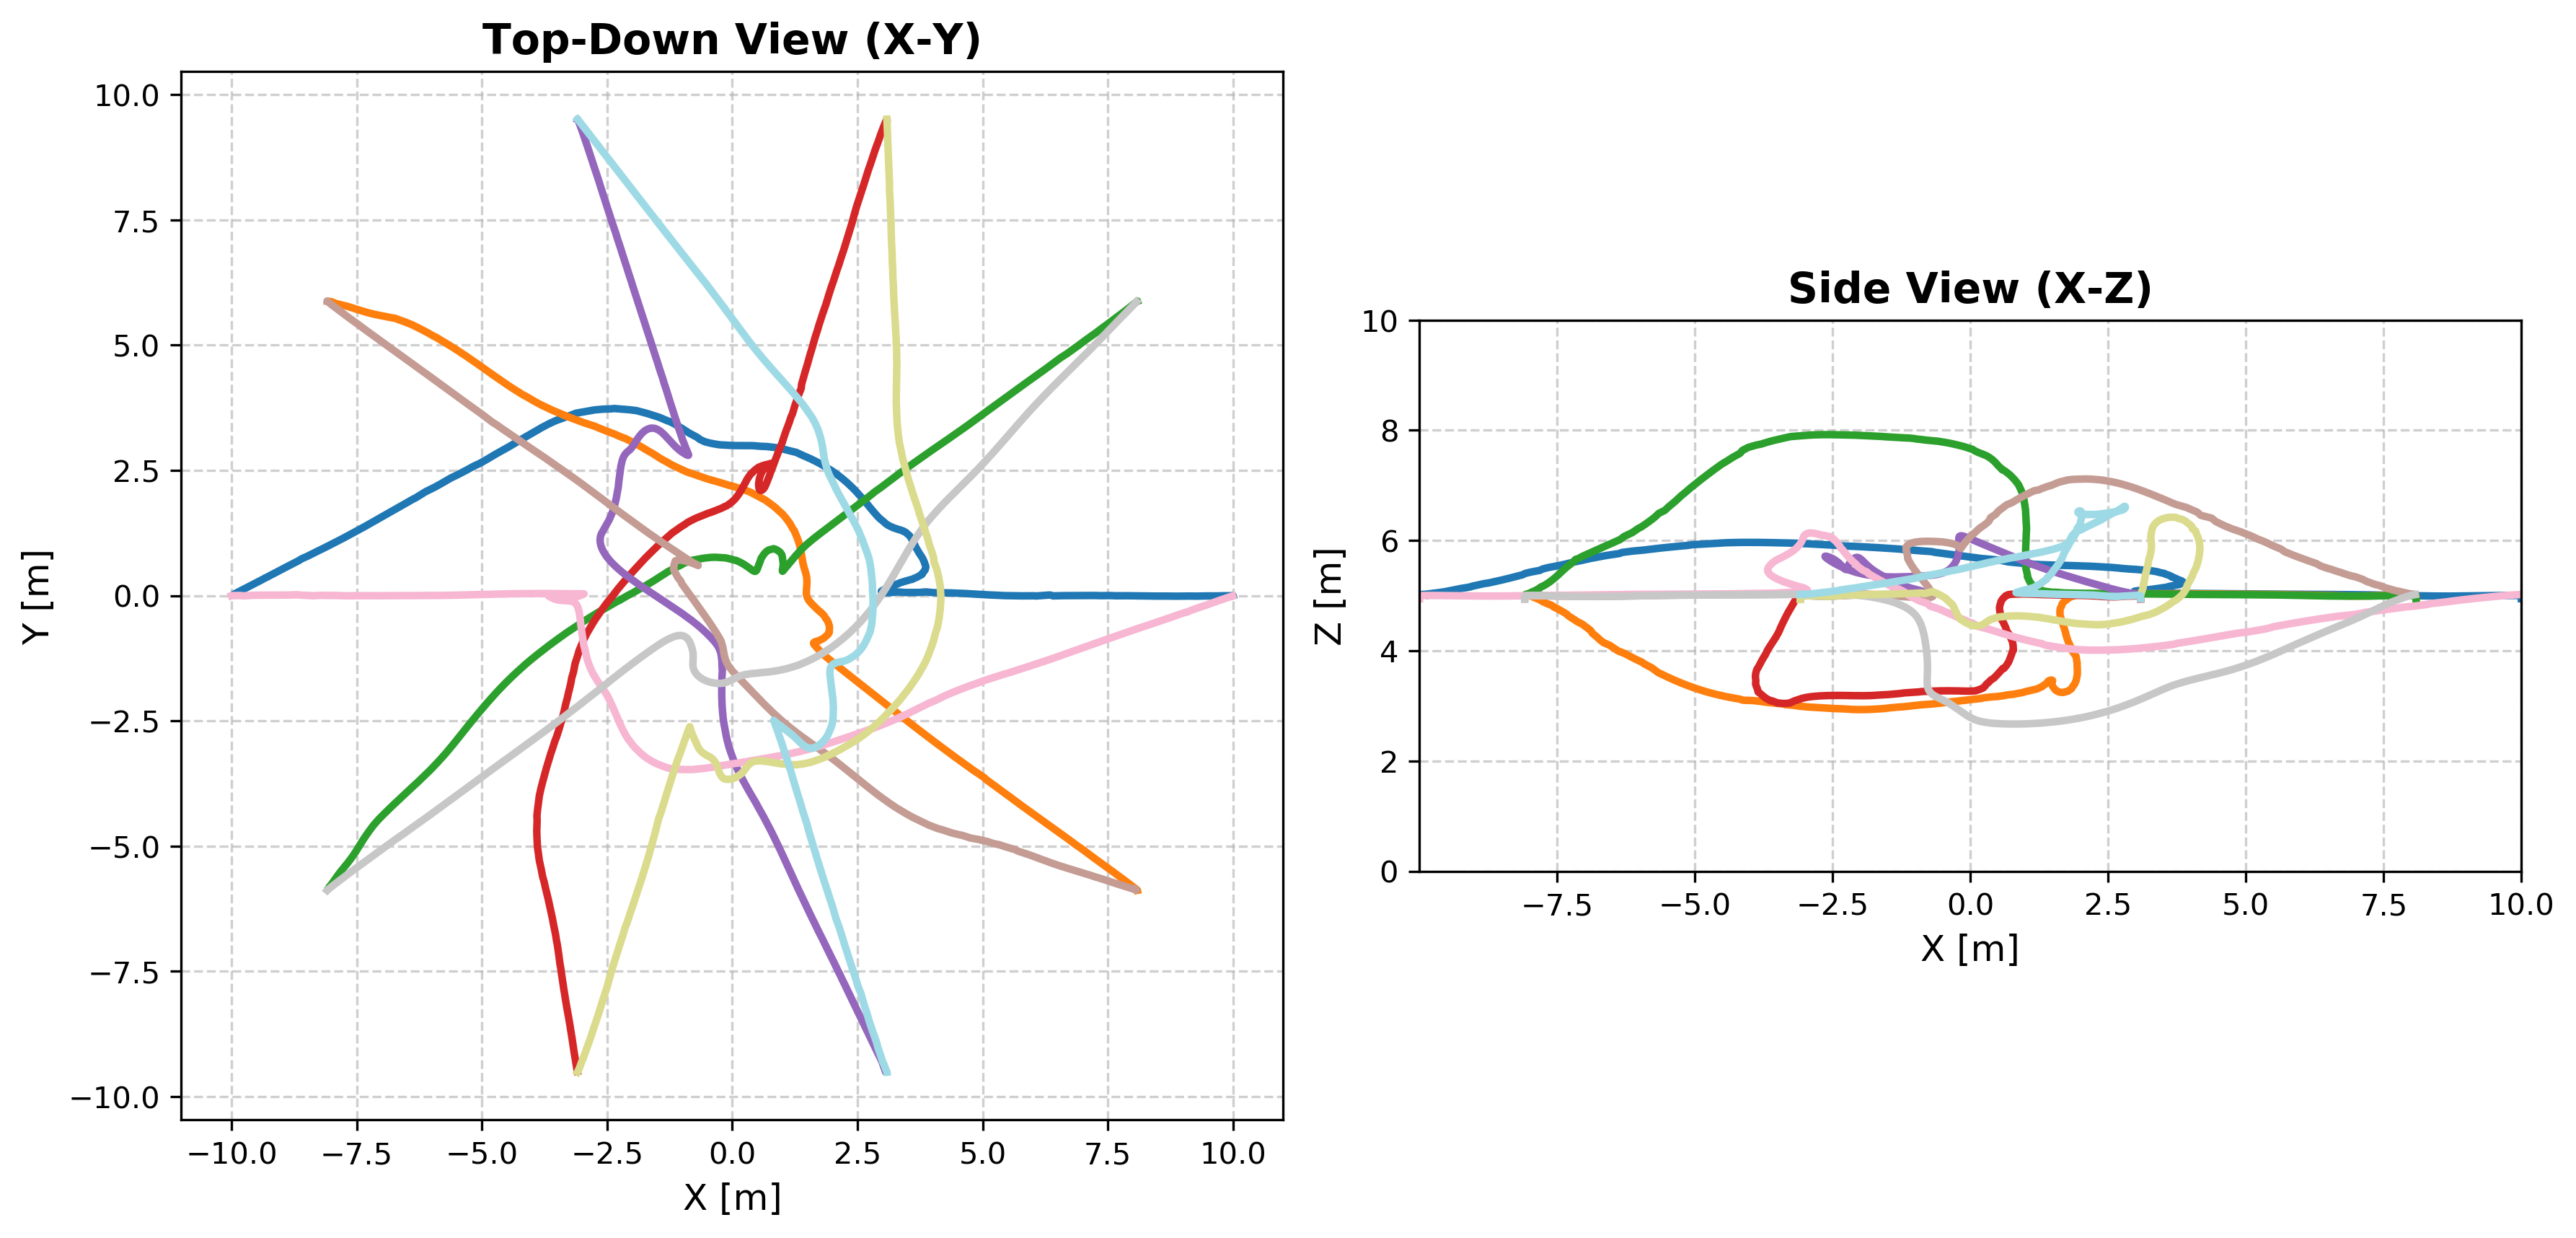
\includegraphics[width=0.48\textwidth, height=0.24\textwidth]{./fig/plots/n_10_circle_z_clipp.png}
                \label{fig:n_10_circle_z_clipp}
            }
            \subfloat[Trajectories of \ac{UAV}s using \ac{3D} \ac{RBL} and using $Z_{rule}$, $N=10$] {
                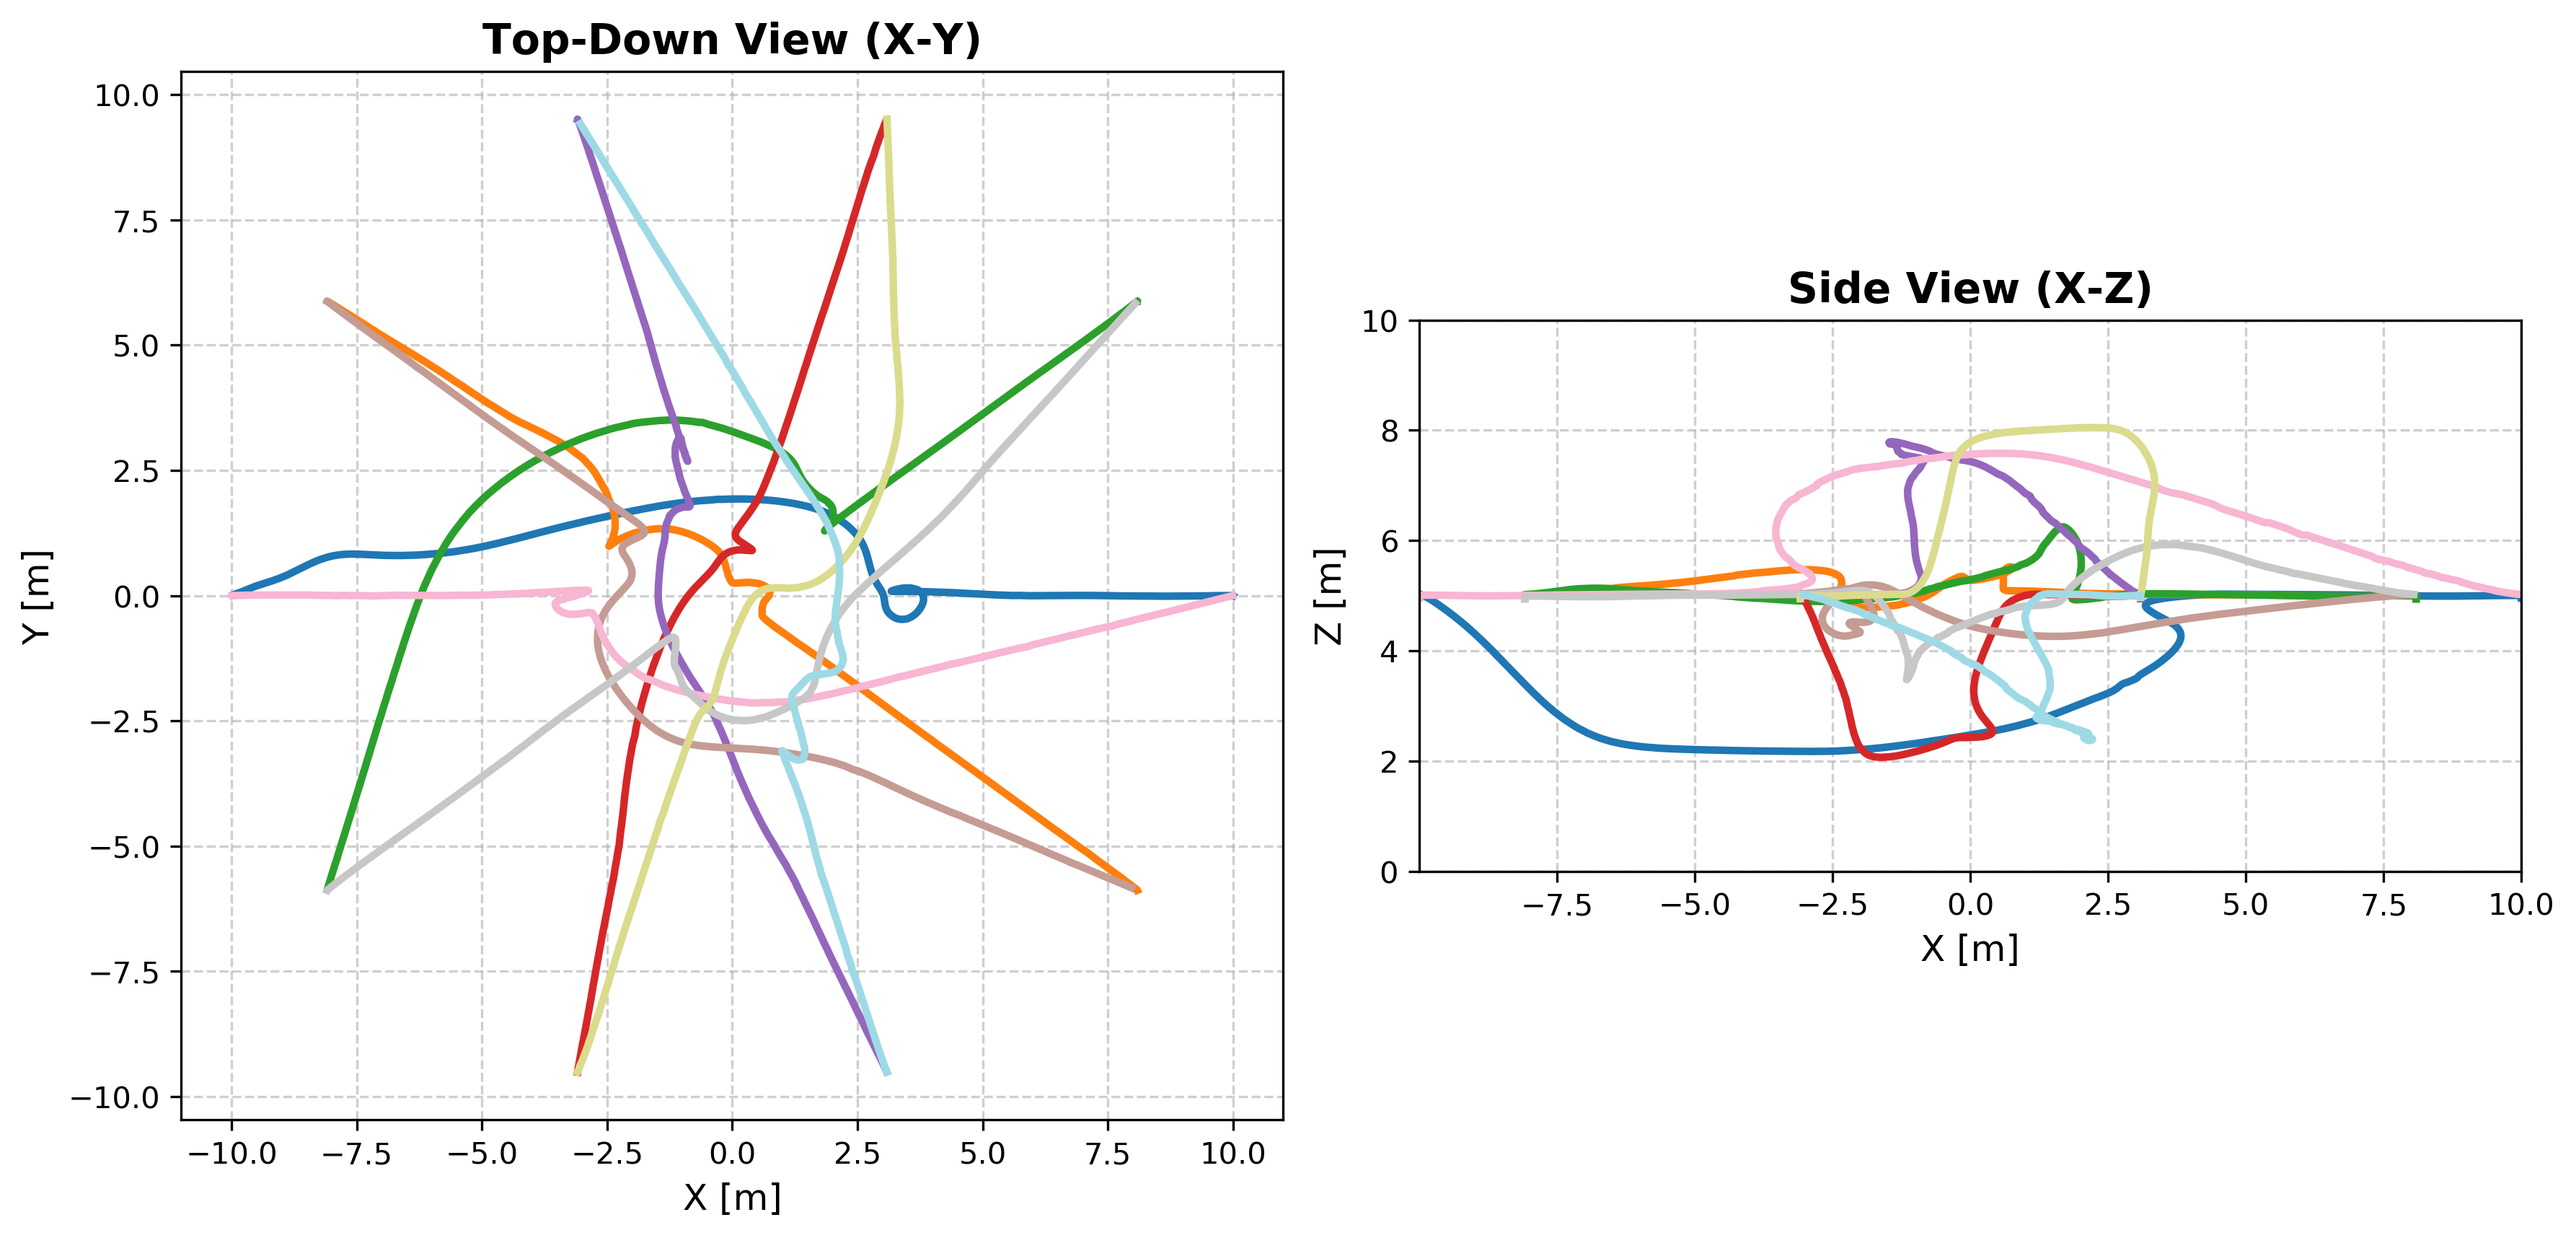
\includegraphics[width=0.48\textwidth, height=0.24\textwidth]{./fig/plots/n_10_circle_z_rule.png}
                \label{fig:n_10_circle_z_rule}
            }
            \par\medskip
            \subfloat[Trajectories of \ac{UAV}s using \ac{3D} \ac{RBL} on sphere, $N=10$] {
                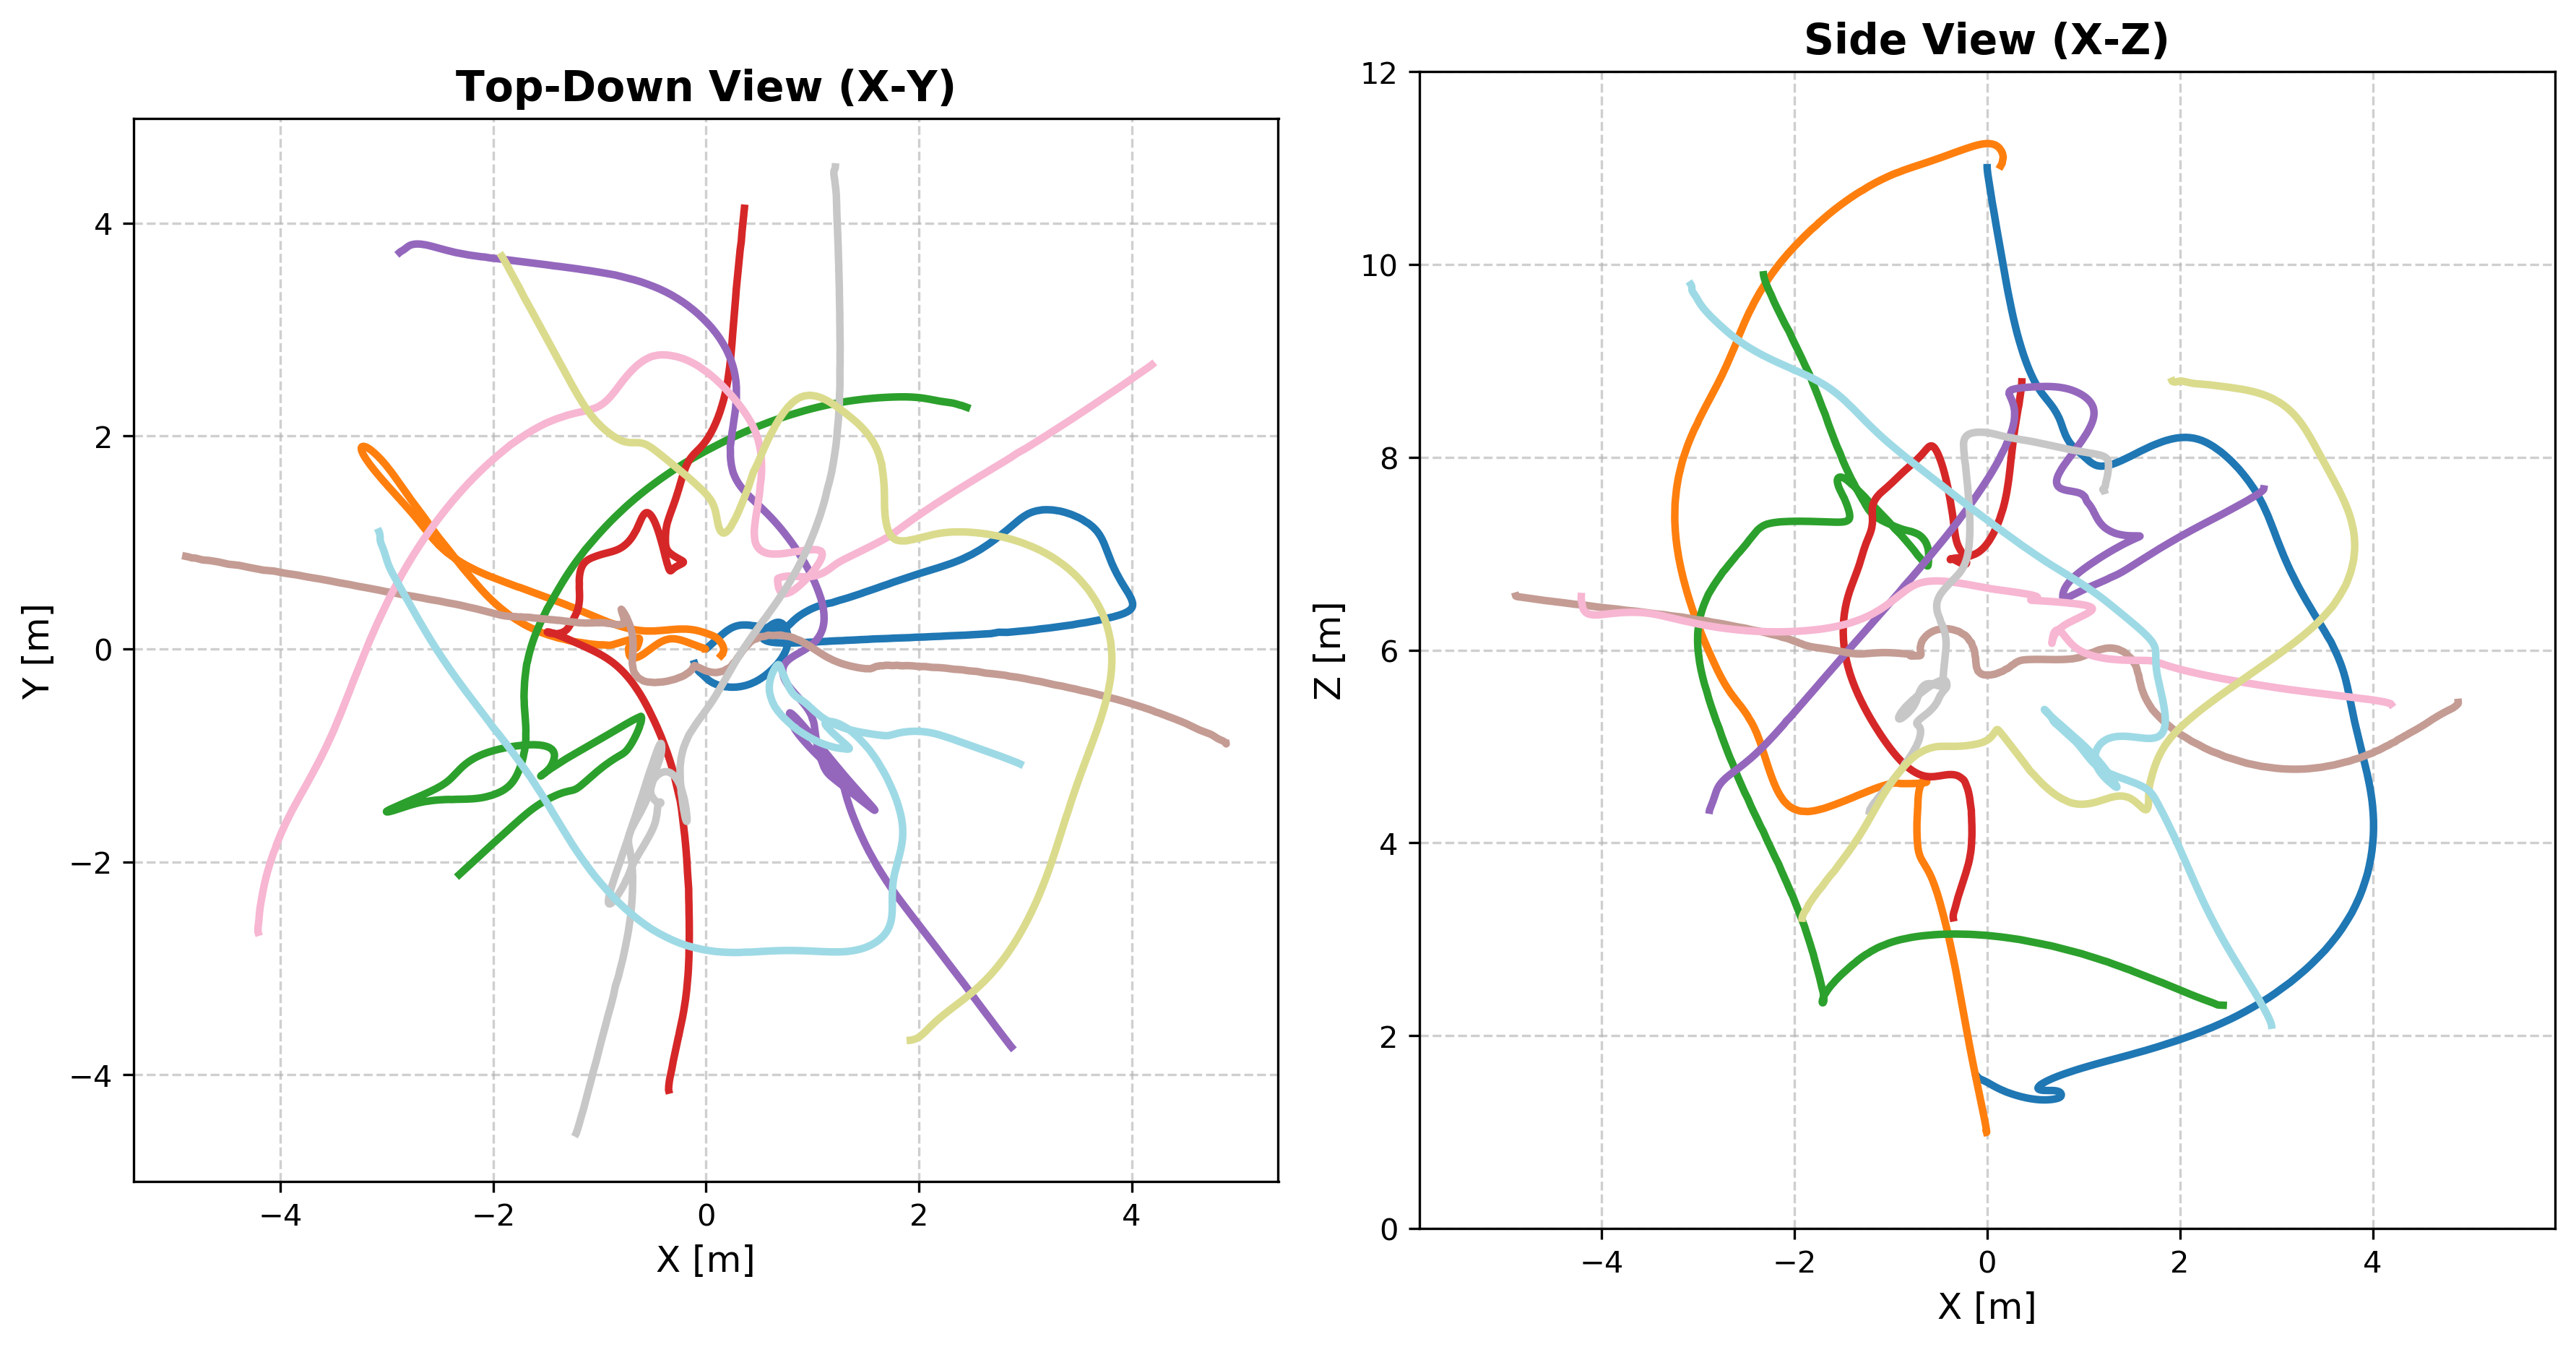
\includegraphics[width=0.48\textwidth, height=0.24\textwidth]{./fig/plots/n_10_sphere.png}
                \label{fig:n_10_sphere}
            }
            \caption{
                Visualization of UAV formations and algorithm behavior for $N=10$ (shown with top-down and side views). 
                (a) Trajectories in a \ac{2D} circular crossing. 
                (b) Trajectories in a \ac{3D} circular crossing. 
                (c) Effect of Z-axis clipping on the circular crossing. 
                (d) Effect of the Z-axis rule on the circular crossing. 
                (e) Trajectories in a \ac{3D} spherical crossing.
            }
            \label{fig:trajectories}
        \end{figure}

    \section{Comparison with State-of-the-Art Method}
        As an alternative approach developed within the MRS framework, the \ac{3D} \ac{RBL} algorithm presented here can be compared to other state-of-the-art methods like PACNav \cite{PACNav}.
        Both algorithms target communication-less UAV coordination, a feature desirable for scalability. 
        Furthermore, implementations described for both approaches have utilized UVDAR to determine the positions of neighbouring UAVs.

        A key requirement for both is some form of self-position estimation. 
        PACNav achieves this in GNSS-denied settings using SLAM techniques. 
        Similarly, \ac{RBL} can also operate without GNSS provided a robust odometry source like SLAM is available to determine the UAV's own position within a consistent frame.

        Where the approaches differ notably is in their coordination strategy. 
        PACNav utilizes a leader-follower dynamic: 'uninformed' UAVs identify and follow 'informed' (or otherwise reliable) leaders based on observed motion characteristics like path persistence and similarity, encouraging group cohesion. 
        In contrast, the RBL algorithm assigns an individual goal to each UAV. 
        Coordination emerges as each agent calculates its path based on its local modified Voronoi cell, moving towards its computed centroid while implicitly accounting for neighbours.

        Regarding validation, PACNav has demonstrated performance through real-world experiments, including navigation in a forest environment. 
        Validation of the multi-agent \ac{3D} RBL algorithm was conducted through simulation.
        The integration and experimental validation of \ac{3D} LiDAR for environmental perception and single-agent navigation within the RBL framework are addressed in the subsequent chapter.

        Another distinct approach in decentralized, communication-less coordination is the purely vision-based model presented by Mezey \cite{mezey_pure_vision}
        Unlike RBL, which relies on explicit position information, the Mezey et al. model derives control actions from a 1D visual projection field generated by detecting neighbours via onboard camera. 
        It requires no localization data. Coordination emerges from low-level visual attraction-repulsion forces, resulting in patterns like flocking or swarming rather than directed motion towards individual goals. 
        While effectively demonstrated in \ac{2D} with \ac{UGV}s, extending this purely vision-based model to complex \ac{3D} environments presents challenges regarding goal achievement. 
        Furthermore, the use of toroidal simulation environments, which mitigate group fragmentation and can facilitate specific emergent patterns like leader-follower dynamics, potentially limits the direct applicability of some observed behaviors to real-world \ac{3D} scenarios.
        The \ac{3D} RBL, by utilizing explicit position information, aims for more predictable goal-oriented navigation in \ac{3D}, although with different sensing requirements compared to the purely reactive, vision-only model of Mezey et al. 
                
    \section{Summary and Key Insights}
        This chpater detailed teh extension of \ac{RBL} algorithm, originally tested for \ac{2D} coordination, to operate in a full three-dimensional space.
        Key modification included adapting The Voronoi cell partitioning for \ac{3D}, utilizing projections for already existing azimuth update rules, and introducing a new elevation rotation angle.
        This new rule dynamically adjusts the agent's vertical destination based on relative centroid positions and directional influence towards the goal, aiming to imporve distribution.
        Note that for the directional influence to work the \ac{UAV}s need to have some sort of information about frame of reference between each other at the start of the algorithm, such as Earth's magnetic field.
        Vertical movement has also been constrained within defined interval ($min_z$, $max_z$).

        The proposed \ac{3D} RBL extensions were evaluated through simulations within the MRS framework, comparing performance \ac{UAV}s crossing circle and sphere. 
        The results indicate that the extension variants successfully enabled multi-agent coordination in three dimensions.
        Specifically, analysis of the simulation results reveals a trend where the performance of the \ac{3D} approach with applied rules compared to the basic \ac{2D} appears to increase with scaling number of agents. 
        For instance, based on the average completion times, the \ac{3D} variant was calculated to be aproximately 1.99\% faster than the \ac{2D} variant for N=5 agents.
        This performance is scales for larger swarms.
        For N=15 the \ac{3D} approach was calculated to be 4.22\% faster than the \ac{2D}.
        This suggests that the extension becomes increasingly beneficial in more crowded scenarios.

        While the magnitude of this observed improvement was perhaps less than initially anticipated, it is important to consider the conservative motion constraints for \ac{UAV}s on the Z-axis (velocity/acceleration), reflecting realistic \ac{UAV} dynamics but limiting vertical exploration.
        Furthermore, the parameters used for testing simulation were also conservative, suggesting that finer tuning - particularly of vertical exploration weights and weighting function agressiveness - could potentially yield better performance.
        Nonetheless, the trend indicated by these results supports the conclusion that the \ac{3D} extension effectiveness crowdeness rises.
        Furthermore, simulations in the spherical formation scenario confirmed the algorithm's capability to manage \ac{3D} navigation and coordination.

        In conclusion, the simulations presented in this chapter demonstrate the feasibility of extending the RBL algorithm to \ac{3D}. 
        The introduced elevation control rule appears particularly beneficial, enhancing the efficiency and convergence speed of the agents towards their goals in simulated \ac{3D} environments. 
        This provides a promising foundation for applying the \ac{3D} RBL algorithm to real-world UAV navigation tasks, explored further in subsequent chapter.


